\documentclass[hidelinks]{article}
\usepackage[english]{babel} 
\usepackage[utf8x]{inputenc}
%% Hyperlinks 
\usepackage{hyperref}
\hypersetup{
    colorlinks,
    linkcolor={red!50!black},
    citecolor={blue!50!black},
    linktoc=all,
    urlcolor={blue!80!black}
}
%% Graphics
\usepackage{graphicx}
\usepackage{float}

\usepackage{enumerate}
\usepackage{multicol}
% Math packages
\usepackage{amsmath}
\usepackage{amssymb}
\usepackage{bm}

% Algorithms
\usepackage{algorithm}
\usepackage[noend]{algpseudocode}
\newcommand\Let[2]{\State #1 $\gets$ #2}
\algrenewcomment[1]{\(\qquad \triangleright\) #1}
\newcommand\Blet[2]{\State \textbf{let} #1 \textbf{be} #2}
\errorcontextlines\maxdimen
% begin vertical rule patch for algorithmicx
% borrowing from http://tex.stackexchange.com/questions/41956/marking-conditional-versions-with-line-in-margin
% see http://tex.stackexchange.com/questions/110431/ploblems-with-vertical-lines-in-algorithmicx
\RequirePackage{zref-abspage}
\RequirePackage{zref-user}
\RequirePackage{tikz}
%\RequirePackage{atbegshi}
%\usetikzlibrary{calc}
\RequirePackage{tikzpagenodes}
\RequirePackage{etoolbox}
\makeatletter
\newcommand*\ALG@lastblockb{b}
\newcommand*\ALG@lastblocke{e}
\apptocmd{\ALG@beginblock}{%
    %\typeout{beginning block, nesting level \theALG@nested, line \arabic{ALG@line}}%
    \ifx\ALG@lastblock\ALG@lastblockb
        \ifnum\theALG@nested>1\relax\expandafter\@firstoftwo\else\expandafter\@secondoftwo\fi{\ALG@tikzborder}{}%
    \fi
    \let\ALG@lastblock\ALG@lastblockb%
}{}{\errmessage{failed to patch}}

\pretocmd{\ALG@endblock}{%
    %\typeout{ending block, nesting level \theALG@nested, line \arabic{ALG@line}}%
    \ifx\ALG@lastblock\ALG@lastblocke
        \addtocounter{ALG@nested}{1}%
        \addtolength\ALG@tlm{\csname ALG@ind@\theALG@nested\endcsname}%
        \ifnum\theALG@nested>1\relax\expandafter\@firstoftwo\else\expandafter\@secondoftwo\fi{\endALG@tikzborder}{}%
        \addtolength\ALG@tlm{-\csname ALG@ind@\theALG@nested\endcsname}%
        \addtocounter{ALG@nested}{-1}%
    \fi
    \let\ALG@lastblock\ALG@lastblocke%
}{}{\errmessage{failed to patch}}
\tikzset{ALG@tikzborder/.style={line width=0.5pt,black}}
\newcommand*\currenttextarea{current page text area}
\newcommand*{\updatecurrenttextarea}{%
    \if@twocolumn
        \if@firstcolumn
            \renewcommand*{\currenttextarea}{current page column 1 area}%
        \else
            \renewcommand*{\currenttextarea}{current page column 2 area}%
        \fi
    \else
        \renewcommand*\currenttextarea{current page text area}%
    \fi
}
\newcounter{ALG@tikzborder}
\newcounter{ALG@totaltikzborder}
\newenvironment{ALG@tikzborder}[1][]{%
    % Allow user to overwrite the used style locally
    \ifx&#1&\else
        \tikzset{ALG@tikzborder/.style={#1}}%
    \fi
    \stepcounter{ALG@totaltikzborder}%
    \expandafter\edef\csname ALG@ind@border@\theALG@nested\endcsname{\theALG@totaltikzborder}%
    \setcounter{ALG@tikzborder}{\csname ALG@ind@border@\theALG@nested\endcsname}%
    %\typeout{begin ALG border nesting level=\theALG@nested, tikzborder=\theALG@tikzborder, tlm=\the\ALG@tlm}%
    \tikz[overlay,remember picture] \coordinate (ALG@tikzborder-\theALG@tikzborder);% node {\theALG@tikzborder};% Modified \tikzmark macro
    \zlabel{ALG@tikzborder-begin-\theALG@tikzborder}%
    % Test if end-label is at the same page and draw first half of border if not, from start place to the end of the page
    \ifnum\zref@extract{ALG@tikzborder-begin-\theALG@tikzborder}{abspage}=\zref@extract{ALG@tikzborder-end-\theALG@tikzborder}{abspage} \else
        \updatecurrenttextarea
        \ALG@drawvline{[shift={(0pt,.5\ht\strutbox)}]ALG@tikzborder-\theALG@tikzborder}{\currenttextarea.south east}{\ALG@thistlm}%
        % If it spreads over more than two pages:
        \newcounter{ALG@tikzborderpages\theALG@tikzborder}%
        \setcounter{ALG@tikzborderpages\theALG@tikzborder}{\numexpr-\zref@extract{ALG@tikzborder-begin-\theALG@tikzborder}{abspage}+\zref@extract{ALG@tikzborder-end-\theALG@tikzborder}{abspage}}%
        \ifnum\value{ALG@tikzborderpages\theALG@tikzborder}>1
            \edef\nextcmd{\noexpand\AtBeginShipoutNext{\noexpand\ALG@tikzborderpage{\theALG@tikzborder}{\the\ALG@thistlm}}}%some pages need a border on the whole page
            \nextcmd
        \fi
    \fi
}{%
    \setcounter{ALG@tikzborder}{\csname ALG@ind@border@\theALG@nested\endcsname}%
    %\typeout{end ALG border nesting level=\theALG@nested, tikzborder=\theALG@tikzborder, tlm=\the\ALG@tlm}%
    \tikz[overlay,remember picture] \coordinate (ALG@tikzborder-end-\theALG@tikzborder);% node {\theALG@tikzborder};% Modified \tikzmark macro
    \zlabel{ALG@tikzborder-end-\theALG@tikzborder}%
    % Test if begin-label is at the same page and draw whole border if so, from start place to end place
    \updatecurrenttextarea
    \ifnum\zref@extract{ALG@tikzborder-begin-\theALG@tikzborder}{abspage}=\zref@extract{ALG@tikzborder-end-\theALG@tikzborder}{abspage}\relax
        \ALG@drawvline{[shift={(0pt,.5\ht\strutbox)}]ALG@tikzborder-\theALG@tikzborder}{ALG@tikzborder-end-\theALG@tikzborder}{\ALG@thistlm}%
    % Otherwise draw second half of border, from the top of the page to the end place
    \else
        %\settextarea
        \ALG@drawvline{\currenttextarea.north west}{ALG@tikzborder-end-\theALG@tikzborder}{\ALG@thistlm}%
    \fi
}
\newcommand*{\ALG@drawvline}[3]{%#1=from, #2=to, #3=value of \ALG@tlm/\ALG@thisthm
    \begin{tikzpicture}[overlay,remember picture]
        \draw [ALG@tikzborder]
            let \p0 = (\currenttextarea.north west), \p1=(#1), \p2 = (#2)
             in
            (#3+\fboxsep+.5\pgflinewidth+\x0,\y1+\fboxsep+.5\pgflinewidth)%-\fboxsep-.5\pgflinewidth
             --
            (#3+\fboxsep+.5\pgflinewidth+\x0,\y2-\fboxsep-.5\pgflinewidth)
            %node[midway,anchor=east] {\ALG@tikzbordertext}
        ;
    \end{tikzpicture}%
}
\newcommand{\ALG@tikzborderpage}[2]{%the whole page gets a border, #1=value of \theALG@tikzborder, #2=value of \ALG@tlm/\ALG@thistlm
    \updatecurrenttextarea
    \setcounter{ALG@tikzborder}{#1}%
    \ALG@drawvline{\currenttextarea.north west}{\currenttextarea.south east}{#2}%
    \addtocounter{ALG@tikzborderpages\theALG@tikzborder}{-1}%
    \ifnum\value{ALG@tikzborderpages\theALG@tikzborder}>1
        \AtBeginShipoutNext{\ALG@tikzborderpage{#1}{#2}}%
    \fi
    \vspace{-0.5\baselineskip}% Compensate for the generated extra space at begin of the page. No idea why exactly this happens.
}
\def\ALG@tikzbordertext{\the\ALG@tlm}
% end vertical rule patch for algorithmicx

% continuation indent patch, slightly extended from http://tex.stackexchange.com/questions/78776/forced-indentation-in-algorithmicx to support multiple paragraphs in one block
\makeatletter
\newlength{\ALG@continueindent}
\setlength{\ALG@continueindent}{2em}
\newcommand*{\ALG@customparshape}{\parshape 2 \leftmargin \linewidth \dimexpr\ALG@tlm+\ALG@continueindent\relax \dimexpr\linewidth+\leftmargin-\ALG@tlm-\ALG@continueindent\relax}
\newcommand*{\ALG@customparshapex}{\parshape 1 \dimexpr\ALG@tlm+\ALG@continueindent\relax \dimexpr\linewidth+\leftmargin-\ALG@tlm-\ALG@continueindent\relax}
\apptocmd{\ALG@beginblock}{\ALG@customparshape\everypar{\ALG@customparshapex}}{}{\errmessage{failed to patch}}
\makeatother
% end continuation indent patch
\usepackage{mathtools}

% Proof system
\usepackage{amsthm}
% spacing fixes for proof system
\makeatletter
\def\thm@space@setup{%
  \thm@preskip=\parskip \thm@postskip=0pt
}
\makeatother
\theoremstyle{plain}
\newtheorem{thm}{Theorem}[section]
\newtheorem{lem}[thm]{Lemma}
\newtheorem{prop}[thm]{Proposition}
\newtheorem{cor}[thm]{Corollary}
\theoremstyle{definition}
\newtheorem{defn}[thm]{Definition}
\newtheorem{exmpl}[thm]{Example}
\newtheoremstyle{rem} % name
    {\topsep}                    % Space above
    {\topsep}                    % Space below
    {}                   % Body font
    {}                           % Indent amount
    {\bf}                   % Theorem head font
    {:}                          % Punctuation after theorem head
    {.5em}                       % Space after theorem head
    {}  % Theorem head spec (can be left empty, meaning ‘normal’)
\theoremstyle{rem}
\newtheorem*{remark}{Note}

% Seitenränder
\usepackage[margin=1.5in]{geometry}
% citations
\usepackage{cite}
% Graphs
\usetikzlibrary{calc,arrows.meta,positioning}
\usepackage{tikz-3dplot}
\usepackage{subfig}
\usepackage{pgfplots}
\pgfplotsset{%
    ,compat=1.12
    ,every axis x label/.style={at={(current axis.right of origin)},anchor=north west}
    ,every axis y label/.style={at={(current axis.above origin)},anchor=north east}
    }

% Notes
\usepackage{xargs} % Use more than one optional parameter in a new commands
\usepackage{xcolor}  % Coloured text etc.
\usepackage[colorinlistoftodos,prependcaption,textsize=tiny]{todonotes}

% absolute text block
\usepackage[absolute]{textpos}
\usepackage{framed}

% Custom commands
\DeclareMathOperator*{\argmin}{arg\,min}
\newcommand{\mx}{\mathcal{X}}
\newcommand{\inp}{\mathcal{I}}
\newcommand{\costs}{c}
\newcommand{\opcosts}{c_{op}}
\newcommand{\swcosts}{c_{sw}}
\newcommand{\fromto}[2]{\{#1,\ldots,#2\}}
\newcommand{\dotcup}{\mathbin{\mathaccent\cdot\cup}}
\newcommandx{\unsure}[2][1=]{\todo[linecolor=red,backgroundcolor=red!25,bordercolor=red,#1]{#2}}
%\newcommandx{\unsure}[2][1=]{}

\pagestyle{plain}
%Title page settings
\usepackage[affil-it]{authblk}

% Title of document
\title{\textbf{Algorithms for Dynamic Right-Sizing\\in Data Centers}}
% Author
\author{Kevin Kappelmann}
\affil{Chair for Theoretical Computer Science,\\ Technical University of Munich}
\date{\today}

% Line breaks after paragraph
\usepackage[parfill]{parskip}
% double line spacing
%\linespread{1.5}

%------------------------------------------------------------------------------
\begin{document}
\pagenumbering{gobble}
\maketitle
\newpage
\begingroup\hypersetup{linkcolor=black}
\tableofcontents
\endgroup 
\newpage

\pagenumbering{arabic}

\section{Introduction}
TODO: Hardware prices vs.\ energy costs in data centres, related work and purpose of this paper (offline algorithm, approximation algorithm,\ldots).

\subsection{Model description}\label{sec_model_descr}
We want to address the issue of above-mentioned ever-growing energy consumption by examining a scheduling problem that commonly arises in data centres. More specifically, we consider a model consisting of a fixed amount of homogeneous servers denoted by $m\in\mathbb{N}$ and a fixed amount of time slots denoted by $T\in\mathbb{N}$. In turn, each server possesses two power states, i.e.\ each server is either powered on (\textit{active state}) or powered off (\textit{sleep state}).
	
For any time slot $t\in[T]$, we have a \textit{mean arrival rate} denoted by $\lambda_t$, i.e.\ the amount of expected load to process in time slot $t$. We expect the arrival rates to be normalised such that each server can handle a load between 0 and 1 in any time slot. We denote the assigned load for server $i$ in time slot $t$ by $\lambda_{i,t}\in[0,1]$. Consequently, for any time slot $t$, we expect an arrival rate between 0 and $m$, that is $\lambda_t\in[0,m]$; otherwise, the servers would not be able to process the given load in time.

The costs incurred by a single machine are described by the sum of the machine's \textit{operating costs}, specified by \makebox{$f:[0,1]\rightarrow \mathbb{R}$}, as well as its \textit{(power state) switching costs}, specified by $\beta\in\mathbb{R}_{\ge 0}$. 
The operating costs $f$ may not exclusively consider energy costs. For example, $f$ may also allow for costs incurred by delays, such as lost revenue caused by users waiting for their responses. Similarly, $\beta$ may also allow for delay costs, wear and tear costs or the like.\cite{dyn_right_size}

We assume that a sleeping server does not cause any costs. Note that $f(0)$ denotes the costs incurred by an idle server, not a sleeping one; in particular, $f(0)$ may be non-zero. Further, we assume convexity for $f$. This may seem like a notable restriction at first, but it indeed captures the behaviour of most modern server models. Since we are dealing with homogeneous servers, $f$ and $\beta$ are the same for all machines.

For convenience, we assume all machines sleeping at time $t=0$ and force all machines to sleep after the scheduling process, i.e.\ at times $t>T$. Consequently, any server must power down exactly as many times as it powers on. This allows us to consolidate power up and power down costs into $\beta$ and to model both costs as being incurred when powering up a server; that is, a model with power up costs $\beta_\uparrow$ and power down costs $\beta_\downarrow$ can be simply transferred to our model by setting $\beta\coloneqq \beta_\uparrow'\coloneqq\beta_\uparrow+\beta_\downarrow$ and $\beta_\downarrow'\coloneqq0$. Similarly, we assume that there are no loads at times $t\notin[T]$, that is $\lambda_t=\lambda_{i,t}=0$ for $t\notin[T]$.

\subsection{Problem statement}
Using above definitions, we can define the input of our model by setting $\inp\coloneqq(m,T,\Lambda,\beta,f)$ where $\Lambda=(\lambda_1,\ldots,\lambda_T)$ is the sequence of arrival rates. We will subsequently identify a problem instance by its input $\inp$. Naturally, given a problem instance $\inp$, we want to schedule our servers in such a way that we minimise the sum of incurred costs while warranting that we are processing the given loads in time.

For this, consider for each server $i\in[m]$ the sequence of its states $S_i$ and the sequence of its assigned loads $L_i$; that is
\begin{align*}
	S_i&\coloneqq(s_{i,1},\ldots,s_{i,T})\in\{0,1\}^T\\
	L_i&\coloneqq(\lambda_{i,1},\ldots,\lambda_{i,T})\in[0,1]^T
\end{align*}
where $s_{i,t}\in\{0,1\}$ denotes whether server $i$ at time $t$ is sleeping (0) or active (1). Recall that we assume all machines sleeping at times $t\notin[T]$; thus, for $t\notin[T]$ and $i\in[m]$, we have $s_{i,t}=0$.

We can now define the sequence of all state changes and the sequence of all assigned loads:
\begin{align*}
	\mathcal{S}&\coloneqq(S_1,\ldots,S_m)\\
	\mathcal{L}&\coloneqq(L_1,\ldots,L_m)
\end{align*}
We will subsequently call a pair $\Sigma\coloneqq(\mathcal{S},\mathcal{L})$ a \textit{schedule}. Finally, we are ready to define our problem statement.

Given an input $\inp$, our goal is to find a schedule $\Sigma$ that satisfies the following optimisation:
\begin{align}
	&\text{minimise}&&\costs(\Sigma)\coloneqq\underbrace{\sum\limits_{t=1}^{T}\sum\limits_{i=1}^{m}\bigl(f(\lambda_{i,t}) s_{i,t}\bigr)}_{\text{operating costs}}+\underbrace{\beta\sum\limits_{t=1}^{T}\sum\limits_{i=1}^{m}\min\{0,s_{i,t}-s_{i,t-1}\}}_{\text{switching costs}}\label{eq_schedule_costs}\\ 
	&\text{subject to}&&\sum\limits_{i=1}^{m}(\lambda_{i,t} s_{i,t})=\lambda_t,\quad \forall t\in[T]\label{eq_feasible_constraint}
\end{align}
We call a schedule \textit{feasible} if it satisfies~\eqref{eq_feasible_constraint} and \textit{optimal} if it satisfies~\eqref{eq_schedule_costs} and~\eqref{eq_feasible_constraint}.
\section{Preliminaries}
In this section, we conduct the preparatory work that will lay the foundations for our algorithms. For this, we analyse the structure of feasible schedules concerning their cost efficiency in order to find characteristics of optimal schedules; these characteristics will then allow us to greatly simplify our optimisation conditions.

We begin by examining the state sequences of feasible schedules. As we are considering homogeneous servers, we do not care which exact servers process the given work loads. Rather we only care about the amount of active servers and the distribution of loads between them. It is in particular unreasonable to power down a machine and to power on a different machine in return; we could just keep the first machine powered on, saving switching costs.
This investigation is captured by our first proposition.
\begin{prop}[Reasonable switching]\label{prop_reasonable_switching}
Given a problem instance $\inp$ and a feasible schedule $\Sigma$, there exists a feasible schedule $\Sigma'$ such that 
\begin{enumerate}[(i)]
		\item $\costs(\Sigma')\le \costs(\Sigma)$ and 
		\item $\Sigma'$ never powers on and shuts down servers at the same time slot, i.e.\ $\Sigma'$ satisfies the following formula:
\begin{equation}
	\forall t\in[T]\Bigl[\bigl(\forall i\in[m](s_{i,t}-s_{i,t-1}\ge0)\bigr)\lor\bigl(\forall i\in[m](s_{i,t}-s_{i,t-1}\le 0)\bigr)\Bigr]\label{eq_reasonable_switching}
\end{equation}
\end{enumerate}
\end{prop}
\begin{proof}
Let $\Sigma=(\mathcal{S},\mathcal{L})$ be a feasible schedule for $\inp$. We give a procedure that repeatedly modifies $\Sigma$ such that it satisfies~\eqref{eq_reasonable_switching} and reduces or retains its costs. 
	
Let $t\in[T]$ be the first time slot falsifying~\eqref{eq_reasonable_switching}. If there does not exist such a time slot, we are done. Otherwise, we can obtain machines $i,j\in[m]$ such that $s_{i,t}-s_{i,t-1}=1$ and \makebox{$s_{j,t}-s_{j,t-1}=-1$}, i.e.\ server $i$ powers on at time $t$ and server $j$ powers off. Without loss of generality, we may assume $i<j$. 
	
First, since all servers are sleeping at time $t=0$, we have
\begin{equation*}
	s_{k,1}-s_{k,0}=s_{k,1}-0=s_{k,1}\ge 0,\quad\forall k\in[m]
\end{equation*}
which satisfies formula~\eqref{eq_reasonable_switching} for $t=1$.
Thus, we may assume $t>1$. 
	
Now consider the state sequences of server $i$ and $j$:
\begin{align*}
	S_i&=(s_{i,1},\ldots,s_{i,t-1}=0,s_{i,t}=1,\ldots,s_{i,T})\\
	S_j&=(s_{j,1},\ldots,s_{j,t-1}=1,s_{j,t}=0,\ldots,s_{j,T})
\end{align*}
We modify $S_i$ and $S_j$ by swapping their states for time slots $\ge t$, that is we set
\begin{align*}
	S_i'&\coloneqq(s_{i,1},\ldots,s_{i,t-1}=0,s_{j,t}=0,\ldots,s_{j,T})\\
	S_j'&\coloneqq(s_{j,1},\ldots,s_{j,t-1}=1,s_{i,t}=1,\ldots,s_{i,T})
\end{align*}
Similarly, we need to swap the assigned loads for server $i$ and $j$:
\begin{align*}
	L_i'&\coloneqq(\lambda_{i,1},\ldots,\lambda_{i,t-1},\lambda_{j,t},\ldots,\lambda_{j,T})\\
	L_j'&\coloneqq(\lambda_{j,1},\ldots,\lambda_{j,t-1},\lambda_{i,t},\ldots,\lambda_{i,T})
\end{align*}
Finally, we construct a new schedule $\Sigma'\coloneqq(\mathcal{S}',\mathcal{L}')$ given by 
\begin{align*}
	\mathcal{S}'&\coloneqq(S_1,\ldots,S_{i-1},S_i',S_{i+1},\ldots,S_{j-1},S_j',S_{j+1},\ldots,S_T)\\
	\mathcal{L}'&\coloneqq(L_1,\ldots,L_{i-1},L_i',L_{i+1},\ldots,L_{j-1},L_j',L_{j+1},\ldots,L_T)
\end{align*}
We want to verify that $\Sigma'$ is a feasible schedule, that is $\Sigma'$ satisfies~\eqref{eq_feasible_constraint}. For time slots $<t$, the schedules $\Sigma'$ and $\Sigma$ still coincide. For time slots $\ge t$, we only changed the order of summation in~\eqref{eq_feasible_constraint}. Thus, $\Sigma'$ is feasible.

Further, $\Sigma$ and $\Sigma'$ coincide in their operating costs; however $\mathcal{S}'$ minimises the switching costs at time $t$. As we assume $\beta\ge0$, we conclude $\costs(\Sigma')\le \costs(\Sigma)$.

Moreover, we decreased the number of servers violating~\eqref{eq_reasonable_switching} at time $t$. Hence, by repeating described process on $\Sigma'$, we obtain a terminating procedure that returns a schedule satisfying the conditions.
\end{proof}

Next, we want to consider the sequence of active servers. For this, let $\mx$ denote the sequence of sums of active servers at each time slot $t$, that is
\begin{equation*}
	\mx\coloneqq\bigl(x_1=\sum\limits_{i=1}^{m}s_{i,1},\ldots,x_T=\sum\limits_{i=1}^{m}s_{i,T}\bigr)\in\fromto{0}{m}^T
\end{equation*}
As we assume all machines sleeping at times $t\notin[T]$, we have $x_t=0$ for $t\notin[T]$.

Our next proposition will require the use of Jensen's inequality, a well-known and frequently used analytic result found by Johan Jensen in 1906.
\begin{lem}[Jensen's inequality]
Let $f:\mathbb{R}\rightarrow\mathbb{R}$ be a convex function, $n\in\mathbb{N}$, \makebox{$\lambda_1,\ldots,\lambda_n\in\mathbb{R}$}, and $\mu_1,\ldots,\mu_n\in[0,1]$ satisfying $\sum\limits_{i=1}^{n}\mu_i=1$. Then the following inequality holds:
\begin{equation*}
	f\Bigl(\sum_{i=1}^n \mu_i \lambda_i\Bigr) \leq \sum_{i=1}^n \mu_i f(\lambda_i)
\end{equation*}
\end{lem}
\begin{proof}
We proof the claim by induction on $n\in\mathbb{N}$.
\begin{itemize}
\item\underline{Basis:} For $n=1$ we have $\mu_1=1$ and thus
\begin{equation*}
	f\Bigl(\sum\limits_{i=1}^1\mu_i\lambda_i\Bigr)=f(\lambda_1)=\sum\limits_{i=1}^1\mu_if(\lambda_i)
\end{equation*}
\item\underline{Step:} Let $n\in\mathbb{N}$ be arbitrary and fixed.
\begin{itemize}
	\item\underline{I.H.:} The assertion holds for $n$.
	\item\underline{Claim:} The assertion holds for $n+1$.
	\item\underline{Proof:} Since $\sum\limits_{i=1}^{n+1}\mu_i=1$, at least one $\mu_i$ must be positive. Without loss of generality, we may assume $\mu_1>0$.
	\begin{equation*}
		f\Bigl(\sum\limits_{i=1}^{n+1}\mu_i\lambda_i\Bigr)=f\Bigl(\mu_1\lambda_1+\sum\limits_{i=2}^{n+1}\mu_i\lambda_i\Bigr)\stackrel{\mu_1\neq 0}{=}f\Bigl(\mu_1\lambda_1+(1-\mu_1)\sum\limits_{i=2}^{n+1}\frac{\mu_i\lambda_i}{1-\mu_1}\Bigr)
	\end{equation*}
	As $f$ is convex, we have
	\begin{equation*}
		f\Bigl(\mu_1\lambda_1+(1-\mu_1)\sum\limits_{i=2}^{n+1}\frac{\mu_i\lambda_i}{1-\mu_1}\Bigr)\stackrel{\text{f convex}}{\le} \mu_1f(\lambda_1)+(1-\mu_1)f\Bigl(\sum\limits_{i=2}^{n+1}\frac{\mu_i\lambda_i}{1-\mu_1}\Bigr)
	\end{equation*}
	Since $\sum\limits_{i=2}^{n+1}\frac{\mu_i}{1-\mu_1}=1$, we can apply our induction hypothesis.
	\begin{equation*}
		\mu_1f(\lambda_1)+(1-\mu_1)f\Bigl(\sum\limits_{i=2}^{n+1}\frac{\mu_i\lambda_i}{1-\mu_1}\Bigr)\stackrel{\text{I.H.}}{\le} \mu_1f(\lambda_1)+(1-\mu_1)\sum\limits_{i=2}^{n+1}\frac{\mu_i}{1-\mu_1}f(\lambda_i)
	\end{equation*}
	We combine our steps and obtain
	\begin{align*}
		f\Bigl(\sum\limits_{i=1}^{n+1}\mu_i\lambda_i\Bigr)&\le \mu_1f(\lambda_1)+(1-\mu_1)\sum\limits_{i=2}^{n+1}\frac{\mu_i}{1-\mu_1}f(\lambda_i)\\
		&=\mu_1f(\lambda_1)+\sum\limits_{i=2}^{n+1}\mu_if(\lambda_i)=\sum_{i=1}^{n+1} \mu_i f(\lambda_i)\qedhere
	\end{align*}
\end{itemize}
\end{itemize}
\end{proof}

The following proposition poses the cornerstone of our subsequent works. We want to establish an optimal scheduling strategy given a fixed amount of active servers. It turns out that an even load distribution seems a very desirable strategy.
\begin{prop}[Even load distribution]\label{prop_even_load_distribution}
Given $x_t\in\mathbb{N}$ active servers in time slot $t$, an arrival rate $\lambda_t\in[0,x_t]$, and a convex cost function $f$, a most cost-efficient and feasible scheduling strategy is to assign each active server a load of $\lambda_t/x_t$.
\end{prop}
\begin{proof}
Let $\Sigma$ be an arbitrary, feasible schedule using $x_t$ servers in time slot $t$, and let $A$ be its set of active servers in time slot $t$, that is $A\coloneqq\{i\in[m]\mid s_{i,t}=1\}$.
Consider the operating costs of $\Sigma$ at time $t$ given by
\begin{equation*}
	\sum\limits_{i=1}^{m}\bigl(f(\lambda_{i,t})\cdot s_{i,t}\bigr)=\sum\limits_{i\in A}\bigl(f(\lambda_{i,t})\cdot1\bigr)+\sum\limits_{i\in [m]\setminus A}\bigl(f(\lambda_{i,t})\cdot0\bigr)=\sum\limits_{i\in A}f(\lambda_{i,t})
\end{equation*}
Since $\Sigma$ is feasible (see constraint~\eqref{eq_feasible_constraint}), we have 
\begin{equation*}
	\sum\limits_{i\in A}\lambda_{i,t}=\lambda_t
\end{equation*}
Hence, we can obtain weights $\mu_1,\ldots,\mu_{x_t}\in[0,1]$ that relate $\lambda_{i,t}$ and $\lambda_t$ for $i\in A$ such that
\begin{align}
	\sum\limits_{i=1}^{x_t}\mu_i=1\quad\text{and}\quad \sum\limits_{i\in A}f(\lambda_{i,t})=\sum\limits_{i=1}^{x_t}f(\mu_i\lambda_t)\label{eq_mu_lambda_costs}
\end{align}
In particular, we have 
\begin{equation}
	\sum_{i=1}^{x_t}\mu_i\lambda_t=\lambda_t\label{eq_mu_convex_comb}
\end{equation}
Using these weights, we now consider the operating costs of a schedule $\Sigma^*$ that evenly distributes $\lambda_t$ to its $x_t$ active servers:
\begin{align*}
	\sum\limits_{i=1}^{x_t}f\Bigl(\frac{\lambda_t}{x_t}\Bigr)=x_tf\Bigl(\frac{\lambda_t}{x_t}\Bigr)\stackrel{\eqref{eq_mu_convex_comb}}{=}x_tf\Bigl(\sum\limits_{i=1}^{x_t}{\frac{\mu_i\lambda_t}{x_t}}\Bigr)
\end{align*}
With the use of Jensen's inequality and the fact that $\sum_{i=1}^{x_t}(1/x_t)=1$, we can give an upper bound for the costs :
\begin{align*}
	x_tf\Bigl(\frac{\lambda_t}{x_t}\Bigr)\le x_t\sum\limits_{i=1}^{x_t}\frac{1}{x_t}f(\mu_i\lambda_t)=\frac{x_t}{x_t}\sum\limits_{i=1}^{x_t}f(\mu_i\lambda_t)=\sum\limits_{i=1}^{x_t}f(\mu_i\lambda_t)\stackrel{\eqref{eq_mu_lambda_costs}}{=}\sum\limits_{i\in A}f(\lambda_{i,t})
\end{align*}
Thus, the operating costs of $\Sigma^*$ give a lower bound for the operating costs of $\Sigma$, and the claim follows.
\end{proof}
As a special case, we can apply our just derived proposition to optimal schedules.
\begin{cor}\label{cor_even_load_distribution}
Given a problem instance $\inp$, there exists an optimal schedule $\Sigma^*$ that evenly distributes its arrival rates to its active servers in each time slot.
\end{cor}
\begin{proof}
Let $\Sigma=(\mathcal{S},\mathcal{L})$ be an optimal schedule for $\inp$. We exchange $\mathcal{L}$ with a new strategy $\mathcal{L}^*$ that evenly distributes the arrival rates to all active servers of $\Sigma$ in each time slot. Setting $\Sigma^*\coloneqq(\mathcal{S},\mathcal{L}^*)$ we have $\costs(\Sigma^*)=\costs(\Sigma)$ by Proposition~\ref{prop_even_load_distribution}. The claim follows.
\end{proof}
As a result of Corollary~\ref{cor_even_load_distribution}, we can restrict ourselves to finding an optimal schedule that evenly distributes its arrival rates to its active servers. We now combine our results to derive the main theorem of our preliminary work.
\begin{thm}\label{thm_even_load_distribution_reasonable_switching}
Given a problem instance $\inp$, there exists an optimal schedule $\Sigma^*$ that evenly distributes its arrival rates to its active servers in each time slot and further satisfies~\eqref{eq_reasonable_switching}.
\end{thm}
\begin{proof}
By Corollary~\ref{cor_even_load_distribution}, we obtain an optimal schedule $\Sigma$ that evenly distributes its arrival rates to its active servers. Applying the procedure given in Proposition~\ref{prop_reasonable_switching} to $\Sigma$ yields $\Sigma^*$ that further satisfies~\eqref{eq_reasonable_switching}.
\end{proof}

Theorem~\ref{thm_even_load_distribution_reasonable_switching} allows us to subsequently identify an optimal schedule by its sequence of active servers $\mx$ and thereby to simplify our optimisation conditions~\eqref{eq_schedule_costs} and \eqref{eq_feasible_constraint}. 
For this, given a problem instance $\inp$, we define the operating costs function $\opcosts(x,\lambda)$ that describes the costs incurred by evenly distributing $\lambda$ on $x$ active servers using $f$:
\begin{equation*}
	\opcosts:\fromto{0}{m}\times[0,m]\rightarrow\mathbb{R}\cup\{\infty\},\quad \opcosts(x,\lambda)=\begin{cases}
          0, & \text{if $x=0$}\\
	  x f(\lambda/x), & \text{if $x\ne 0\land\lambda\le x$}\\
	  \infty, & \text{if $x\ne 0\land\lambda>x$}
	  \end{cases} \label{fct:c}
\end{equation*}
We assign infinite costs in case $\lambda>x$ as there would be too few active servers to process the arrival rate, i.e.\ the schedule would not be feasible. Next, we define the switching costs function $\swcosts(x_{t-1},x_t)$ that describes the incurred costs when changing the amount of active server from $x_{t-1}$ to $x_t$:
\begin{equation*}
	\swcosts(x_{t-1},x_t)\coloneqq\beta\max\{0,x_t-x_{t-1}\}
\end{equation*}
Lastly, we can define the costs function $\costs(x_{t-1},x_t,\lambda_t)$ that describes the incurring costs for a single time step using an even distribution of loads:
\begin{equation*}
	\costs(x_{t-1},x_{t},\lambda_t)\coloneqq\opcosts(x_t,\lambda_t)+\swcosts(x_{t-1},x_t)
\end{equation*}
The optimisation conditions for a schedule now simplify to one single minimisation:
\begin{align}
	\text{minimise}\quad \costs(\mx)\coloneqq\sum\limits_{t=1}^{T}\costs(x_{t-1},x_{t},\lambda_t)\label{eq_even_distribution_schedule_costs}
\end{align}
We subsequently call a schedule $\mx$ \textit{optimal} if it satisfies~\eqref{eq_even_distribution_schedule_costs}.

\section{Optimal offline scheduling}
In this section, we derive two optimal offline algorithms based on our preliminary work.
First, we reduce our problem specified by $\inp$ to a shortest path problem of a level structured graph $G$. We then use a dynamic programming approach to find a shortest path in $G$ and thereby an optimal schedule for $\inp$ in pseudo-polynomial time $\Theta(Tm^2)$.
After that, we refine our initial approach to derive an improved algorithm with pseudo-linear complexity $\Theta(Tm)$.

\subsection{A pseudo-polynomial algorithm}\label{sec_opt_offline_pseudo_poly}
Let $\inp$ be a problem instance. Thanks to our preliminary work, we know that there exists an optimal schedule which is identifiable by its sequence of active servers $\mx$. In order to find this sequence $\mx$, consider the weighted, level structured graph $G$ defined as follows:
\begin{align*}
	&V\coloneqq\bigl\{v_{x,t}\mid x\in\fromto{0}{m},t\in[T]\bigr\}\dotcup\{v_{0,0},v_{0,T+1}\}\\
	&E\coloneqq\bigl\{(v_{x,t},v_{x',t+1})\mid x,x'\in\fromto{0}{m},t\in\fromto{0}{T},v_{x,t},v_{x',t+1}\in V\bigr\}\\
	&c_G(v_{x,t},v_{x',t+1})\coloneqq\costs(x,x',\lambda_{t+1})\\
	&G\coloneqq(V,E,c_G)
\end{align*}
For any possible amount of active servers $x$ and any time slot $t$, we add a node $v_{x,t}$. Moreover, we add a start node $v_{0,0}$ as well as an end node $v_{0,T+1}$. Next, we connect all nodes to their successors with respect to time. Semantically, $v_{x,t}$ denotes the state of distributing the arrival rate $\lambda_{t}$ evenly to $x$ servers in time slot $t$. For any edge connecting $v_{x,t}$ with $v_{x',t+1}$, we assign costs $\costs(x,x',\lambda_{t+1})$, i.e.\ the costs of taking the edge correspond to switching from $x$ to $x'$ machines and processing the load $\lambda_{t+1}$ with $x'$ machines. A graphical representation can be found in the following figure.
\begin{figure}[H]
\centering
\scalebox{0.86}{
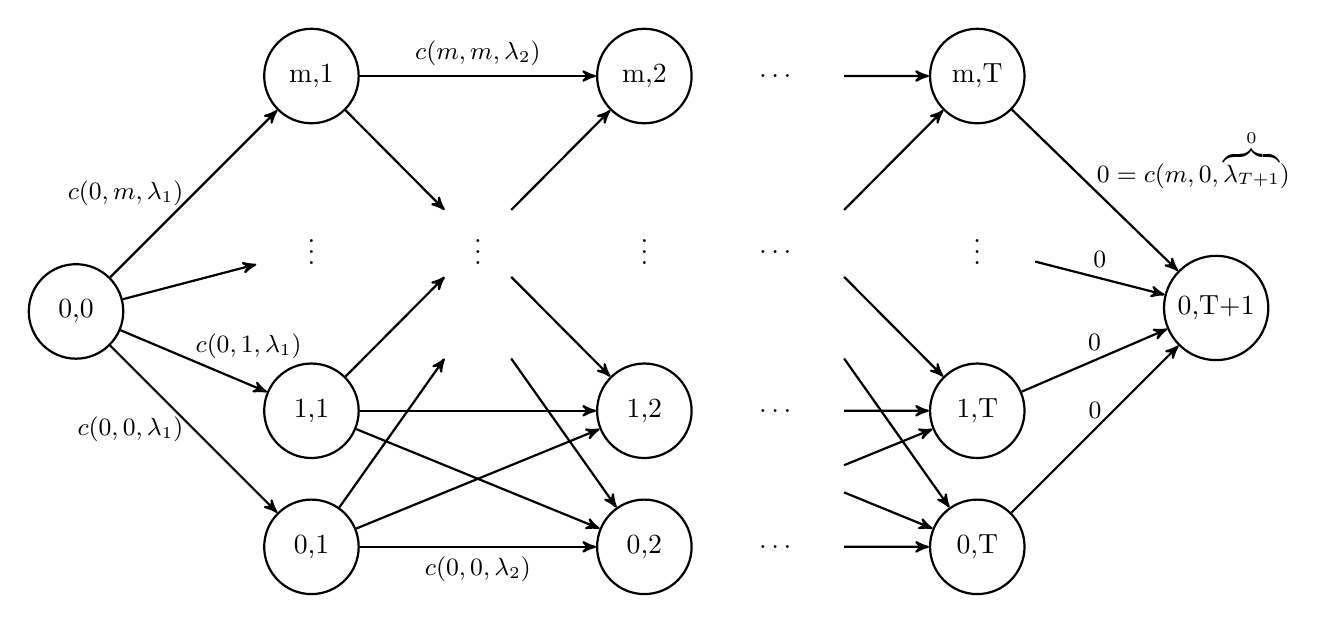
\begin{tikzpicture}[->,>=stealth',auto,node distance=3cm,thick,node/.style={minimum size=1.2cm,circle,draw}]

  \node[node] (1) {0,0};
  \node[node] (4) [below right =of 1] {0,1};
  \node[node] (3) [above =0.5cm of 4] {1,1};
  \node[node] (2) [above right=of 1] {m,1};
  \node[node] (6) [right =of 3] {1,2};
  \node[node] (5) [right =of 2] {m,2};
  \node[node] (7) [right =of 4] {0,2};
  \node[node] (9) [right =of 6] {1,T};
  \node[node] (8) [right =of 5] {m,T};
  \node[node] (10) [right =of 7] {0,T};
  \node[node] (11) [above right =of 10] {0,T+1};

  \node at ($(5)!.4!(8)$) {\ldots};
  \node (12) at ($(6)!.4!(9)$) {\ldots};
  \node at ($(7)!.4!(10)$) {\ldots};
  \node [above=1.72cm of 12]{\ldots};

  \node at ($(2)!.5!(3)$) {\vdots};
  \node at ($(2)!.5!(6)$) {\vdots};
  \node at ($(5)!.5!(6)$) {\vdots};
  \node at ($(8)!.5!(9)$) {\vdots};

  \path[every node/.style={font=\sffamily\small}]
    (1) edge node[left] {$\costs(0,m,\lambda_1)$} (2)
	edge node[above right=-0.15cm] {$\costs(0,1,\lambda_1)$} (3)
	edge node[left] {$\costs(0,0,\lambda_1)$} (4)
    (2) edge node[above] {$\costs(m,m,\lambda_2)$} (5)
    (3) edge (6)
	edge (7)
    (4) edge (6)
	edge node[below] {$\costs(0,0,\lambda_2)$} (7)
    (8) edge node[above right=-0.15cm] {$0=\costs(m,0,\overbrace{\lambda_{T+1}}^{0})$} (11)
    (9) edge node[above] {$0$} (11)
    (10) edge node[above] {$0$} (11)

    (1) edge ($(1)!.2!(8)$)
    (2) edge ($(2)!.4!(6)$)
    (4) edge ($(4)!.4!(5)$)
    (3) edge ($(3)!.4!(5)$)
    ($(3)!.6!(5)$) edge (5)
    ($(2)!.6!(6)$) edge (6)
    ($(2)!.6!(7)$) edge (7)

    ($(6)!.6!(8)$) edge (8)
    ($(5)!.6!(8)$) edge (8)

    ($(5)!.6!(9)$) edge (9)
    ($(6)!.6!(9)$) edge (9)
    ($(7)!.6!(9)$) edge (9)

    ($(5)!.6!(10)$) edge (10)
    ($(6)!.6!(10)$) edge (10)
    ($(7)!.6!(10)$) edge (10)

    ($(2)!.8!(11)$) edge node[above] {$0$} (11);

\end{tikzpicture}
}
\caption{Level structured graph for a pseudo-polynomial, optimal offline algorithm}
\label{fig_graph_pseudo_poly}
\end{figure}
The costs of a path $P=(v_{x_0,T_0},v_{x_1,T_0+1},\ldots,v_{x_n,T_0+n})$ with length $n$ in our graph (where $x_t\in\fromto{0}{m}, T_0\in\fromto{0}{T}$ and $T_0+n\leq T+1$) are thus given by
\begin{equation*}
	\costs(P)\coloneqq\sum\limits_{t=1}^{n}\costs(x_{t-1},x_t,\lambda_{T_0+t})
\end{equation*}
In particular, for a path $P=(v_{0,0},v_{x_1,1},\ldots,v_{x_T,T},v_{0,T+1})$ from our start node $v_{0,0}$ to our end node $v_{0,T+1}$ we have
\begin{equation}
	\costs(P)=\costs(0,x_1,\lambda_1)+\sum\limits_{t=2}^{T}\costs(x_{t-1},x_{t},\lambda_{t})+\underbrace{\costs(x_T,0,0)}_{=0}=\costs(0,x_1,\lambda_1)+\sum\limits_{t=2}^{T}\costs(x_{t-1},x_{t},\lambda_{t})\label{eq_v0_VT1_path_costs}
\end{equation}
Note that the costs of such a path directly correspond to those of a schedule $\mx$ (see~\eqref{eq_even_distribution_schedule_costs}).
Any shortest path from $v_{0,0}$ to $v_{0,T+1}$ is thus forced to minimise the costs of the corresponding schedule. Needless to say, this demands for a proof of correctness.
\begin{lem}\label{lem_sched_path_pseudo_poly}
Let $\bm{\mx}$ be the set of all schedules $\mx$ for $\inp$, and let $\bm{\mathcal{P}}$ the set of all paths from $v_{0,0}$ to $v_{0,T+1}$. The map
\begin{equation*}
	\Phi:\bm{\mathcal{P}}\rightarrow\bm{\mx},\quad (v_{0,0},v_{x_1,1},v_{x_2,2},\ldots,v_{x_T,T},v_{0,T+1})\mapsto (x_1,\ldots,x_T)
\end{equation*}
is a bijection with inverse map
\begin{equation*}
	\Psi:\bm{\mx}\rightarrow\bm{\mathcal{P}},\quad(x_1,\ldots,x_T)\mapsto (v_{0,0},v_{x_1,1},v_{x_2,2},\ldots,v_{x_T,T},v_{0,T+1})
\end{equation*}
satisfying $\costs(\mx)=\costs\bigl(\Psi(\mx)\bigr)$.
\end{lem}
\begin{proof}
It is easy to check that $\Psi\circ\Phi=id_{\bm{\mathcal{P}}}$ and $\Phi\circ\Psi=id_{\bm{\mx}}$. Thus, $\Phi$ is indeed bijective with inverse map $\Psi$. Next, let $\mx=(x_1,\ldots,x_T)$ be a schedule for $\inp$. We have
\begin{equation*}
	P\coloneqq\Psi(\mx)=(v_{0,0},v_{x_1,1},v_{x_2,2},\ldots,v_{x_T,T},v_{0,T+1})
\end{equation*}
We examine the costs of $\mx$ and conclude
\begin{equation*}
\costs(\mx)\stackrel{\eqref{eq_even_distribution_schedule_costs}}{=}\sum\limits_{t=1}^{T}\costs(x_{t-1},x_{t},\lambda_t)=\underbrace{\costs(x_0,x_1,\lambda_1)}_{=\costs(0,x_1,\lambda_1)}+\sum\limits_{t=2}^{T}\costs(x_{t-1},x_{t},\lambda_t)\stackrel{\eqref{eq_v0_VT1_path_costs}}{=}\costs(P)
\end{equation*}
Which shows that $\Psi$ and, as a consequence, $\Phi$ are cost-preserving maps. The claim follows.
\end{proof}
\begin{thm}\label{thm_opt_sched_short_path_pseudo_poly}
There is a cost-preserving bijection between optimal schedules $\mx$ for $\inp$ and shortest paths from $v_{0,0}$ to $v_{0,T+1}$.
\end{thm} 
\begin{proof}
By Lemma~\ref{lem_sched_path_pseudo_poly}, we have a bijection $\Psi$ between schedules $\mx$ and paths from $v_{0,0}$ to $v_{0,T+1}$ obeying $\costs(\mx)=\costs\bigl(\Psi(\mx)\bigr)$. Thus, we have 
\begin{equation*}
	\costs(\mx)\text{ minimal}\iff \costs\bigl(\Psi(\mx)\big)\text{ minimal}
\end{equation*}
and the claim follows.
\end{proof}
In the following, we give an algorithm based on our just verified construction. 
We split our procedure into two subroutines. 

\textproc{shortest\_paths} uses a dynamic programming approach similar to the well-known Bellman-Ford algorithm. It returns the minimum costs to all nodes as well as the predecessor of any node in respect to its shortest path.

\textproc{extract\_schedule} uses the predecessors calculated by \textproc{shortest\_paths} in order to obtain the sequence of nodes describing a shortest path and thereby a schedule for our problem instance.
\begin{algorithm}[H]
  \caption{Pseudo-polynomial optimal offline scheduling}
  \begin{algorithmic}[1]
  \Function{optimal\_offline\_scheduling}{$m,T,\Lambda,\beta,f$}
	  \Let{$(C,P)$}{\Call{shortest\_paths}{$m,T,\Lambda,\beta,f$}}
	  \Let{$\mx$}{\Call{extract\_schedule}{$P,T$}}
	  \State \Return{$\mx$}
  \EndFunction
  \Statex
  \Function{shortest\_paths}{$m,T,\Lambda,\beta,f$}
	\Blet{$C[T+1,m]$ and $P[T+1,m]$}{new arrays}\Comment{Costs and predecessors of nodes}
	\For{$x \gets 0 \textrm{ to } m$}\Comment{Initialisation}
		\Let{$C[1,x]$}{$\costs(0,x,\lambda_1)$}
		\Let{$P[1,x]$}{$0$}
	\EndFor
	\For{$t \gets 2 \textrm{ to } T$}\Comment{Iterative calculation of costs and predecessors}
		\For{$x' \gets 0 \textrm{ to } m$}
			\Let{$P[t,x']$}{$\argmin\limits_{x\in\fromto{0}{m}}\bigl\{C[t-1,x]+\costs(x,x',\lambda_t)\bigr\}$}\Comment{Find best preceding choice}
			\Let{$C[t,x']$}{$C\bigl[t-1,P[t,x']\bigr]+c\bigl(P[t,x'],x',\lambda_t\bigr)$}
		\EndFor
	\EndFor
	\Let{$P[T+1,0]$}{$\argmin\limits_{x\in\fromto{0}{m}}\bigl\{C[T,x]\bigr\}$}\Comment{Find best choice for last time slot}
	\Let{$C[T+1,0]$}{$C\bigl[T,P[T+1,0]\bigr]$}
	\State \Return{$(C,P)$}
  \EndFunction
  \Statex
  \Function{extract\_schedule}{$P,T$}
	\Blet{$\mx[T]$}{a new array}
    	\Let{$\mx[T]$}{$P[T+1,0]$}\Comment{Get best choice for last time slot}
        \For{$t \gets T-1 \textrm{ to } 1$}\Comment{Iteratively obtain a schedule by using the predecessors}
		\Let{$\mx[t]$}{$P\bigl[t+1,\mx[t+1]\bigr]$}
	\EndFor
	\State \Return{$\mx$}
  \EndFunction

  \end{algorithmic}
\label{alg_opt_offline_pseudo_poly}
\end{algorithm}
The correctness of Algorithm~\ref{alg_opt_offline_pseudo_poly} directly follows from the correctness of the Bellman-Ford algorithm and Theorem~\ref{thm_opt_sched_short_path_pseudo_poly}.

Naturally, we are interested in our algorithm's time and memory complexity. Subroutine
\textproc{shortest\_paths} needs $\Theta(m)$ iterations for its initialisation, $\Theta(Tm^2)$ steps for the iterative calculation, and $\Theta(m)$ steps for its final minimisation search. In addition, \textproc{extract\_schedule} needs $\Theta(T)$ iterations for its schedule retrieval. Thus, we receive a runtime of 
\begin{equation*}
	\Theta(m+Tm^2+m+T)=\Theta(Tm^2)
\end{equation*}
The runtime is polynomial in the numeric value of the input; however, as we just need $\log_2(m)$ bits to encode $m$, it is exponential in the length of the input. Hence, the algorithm is pseudo-polynomial.

Our memory demand is defined by the size of the arrays $C$ and $P$. As both arrays are of size $\Theta(Tm)$, we have a memory complexity of $\Theta(Tm)$

\subsection{A pseudo-linear algorithm}\label{sec_opt_offline_pseudo_lin}
The algorithm developed in section~\ref{sec_opt_offline_pseudo_poly} is of a quite simple nature. Its underlying graph $G$ is able to represent any possible schedule $\mx$ since we simply we add an edge for any possible scheduling choice at any possible time slot. This approach seems rather intuitive and readily verifiable, but this convenience comes with a cost; the density of $G$ causes a quadratic runtime in the number of servers $m$. In order to improve the runtime to pseudo-linear complexity, we need to thin out our graph. 

Let us revise our initial algorithm. Our graph consists of nodes $v_{x,t}$. Any node $v_{x,t}$ denotes the state of distributing the arrival rate $\lambda_{t}$ evenly to $x$ servers in time slot $t$. The algorithm calculates the minimum costs to all nodes. The cost of a node $v_{x,t}$ thus corresponds to the lowest achievable cost up to time slot $t$ of all schedules $\mx$ that assign $x$ servers at time $t$ to process the arrival rate $\lambda_t$. In particular, the cost of the end node $v_{0,T+1}$ tell us the minimum cost of all schedules. This approach, however, does not consider the possibility to schedule $y\neq x$ servers in time slot $t$ and to switch to $x$ servers just at the very last moment of $t$ when calculating the cost of $v_{x,t}$. Consider the following example:
\begin{exmpl}
Let $\inp_i=(m=1,T=2,\Lambda_i,\beta=1,f)$ be the inputs for two problem instances with $f(x)=x^2+1$, $\Lambda_1=(1,0)$, and $\Lambda_2=(0,1)$. Below we illustrate the graphs for the two problem instances and the corresponding calculations done by the algorithm derived in section~\ref{sec_opt_offline_pseudo_poly}.
\begin{figure}[H]
\captionsetup{farskip=-1em} 
\captionsetup[subfigure]{labelformat=empty}
\centering
\subfloat[\underline{Problem $\inp_1$:} State $v_{0,1}$ could be reached with cost $3$ by moving down from node $v_{1,1}$.]{
\scalebox{0.75}{
  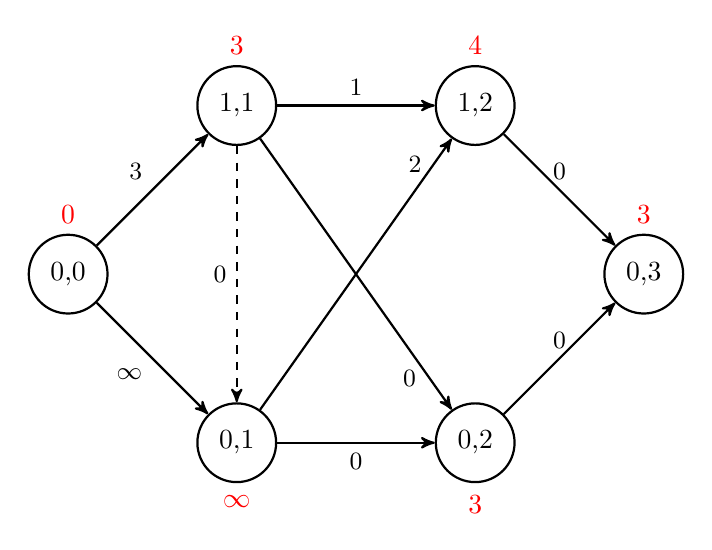
\begin{tikzpicture}[->,>=stealth',auto,node distance=2cm,thick,node/.style={minimum size=1cm,circle,draw}]
  \node[node, label={[color=red]$0$}] (1) {0,0};
  \node[node, label={[below=1.05cm,color=red]$\infty$}] (2) [below right =of 1] {0,1};
  \node[node, label={[color=red]$3$}] (3) [above right=of 1] {1,1};
  \node[node, label={[below=1.05cm,color=red]$3$}] (4) [right =of 2] {0,2};
  \node[node, label={[color=red]$4$}] (5) [right =of 3] {1,2};
  \node[node, label={[color=red]$3$}] (6) [below right =of 5] {0,3};

  \path[every node/.style={font=\sffamily\small}]
    (1) edge node[below left] {$\infty$} (2)
	edge node[above left] {$3$} (3)
    (2) edge node[below] {$0$} (4)
    (2) edge node[label={[xshift=0.88cm, yshift=0.9cm]$2$}] {} (5)
    (3) edge node[label={[xshift=0.55cm, yshift=-1.82cm]$0$}] {} (4)
    (3) edge node[above] {$1$} (5)
    (4) edge node[above] {$0$} (6)
    (5) edge node[above] {$0$} (6)
    (3) edge[dashed] node[left] {$0$} (2);
\end{tikzpicture}
}}
\qquad
\subfloat[\underline{Problem $\inp_2$:} State $v_{1,1}$ could be reached with cost $1$ by moving up from $v_{0,1}$.]{
\scalebox{0.75}{
  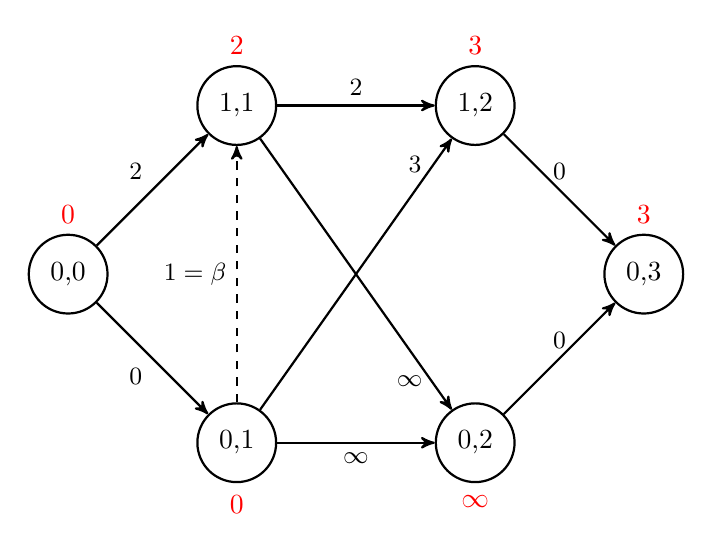
\begin{tikzpicture}[->,>=stealth',auto,node distance=2cm,thick,node/.style={minimum size=1cm,circle,draw}]
  \node[node, label={[color=red]$0$}] (1) {0,0};
  \node[node, label={[below=1.05cm,color=red]$0$}] (2) [below right =of 1] {0,1};
  \node[node, label={[color=red]$2$}] (3) [above right=of 1] {1,1};
  \node[node, label={[below=1.05cm,color=red]$\infty$}] (4) [right =of 2] {0,2};
  \node[node, label={[color=red]$3$}] (5) [right =of 3] {1,2};
  \node[node, label={[color=red]$3$}] (6) [below right =of 5] {0,3};

  \path[every node/.style={font=\sffamily\small}]
    (1) edge node[below left] {$0$} (2)
	edge node[above left] {$2$} (3)
    (2) edge node[below] {$\infty$} (4)
    (2) edge node[label={[xshift=0.88cm, yshift=0.9cm]$3$}] {} (5)
    (3) edge node[label={[xshift=0.55cm, yshift=-1.82cm]$\infty$}] {} (4)
    (3) edge node[above] {$2$} (5)
    (4) edge node[above] {$0$} (6)
    (5) edge node[above] {$0$} (6)
    (2) edge[dashed] node[left] {$1=\beta$} (3);
\end{tikzpicture} }}
\caption{Two examples depicting a shortcoming of our initial approach. The calculated nodes' costs are highlighted in red. Dashed edges are not part of the initial algorithm.}
\end{figure}
\end{exmpl}
Although our algorithm delivers the correct end results, its immediate steps are somewhat unsatisfying. We want our states to capture a more general notion than given in section~\ref{sec_opt_offline_pseudo_poly}; preferably, we would like a node $v_{x,t}$ to denote the state of having $x$ active servers at the end of time slot $t$. In practice, we may reach a state $v_{x,t}$ by moving down from a state $v_{y^\downarrow,t}$ where $y^\downarrow>x$ with cost $0$ or by moving up from a state $v_{y^\uparrow,t}$ where $y^\uparrow<x$ with cost $\beta(x-y^\uparrow)$.

In order to allow for these new possibilities, given a problem instance $\inp$, we define a directed, weighted graph as follows:
\begin{align*}
	&V\coloneqq\bigl\{v_{x,t\downarrow}\mid x\in\fromto{0}{m},t\in[T]\bigr\}\dotcup\bigl\{v_{x,t\uparrow}\mid x\in\fromto{0}{m},t\in[T-1]\bigr\}\dotcup\{v_{0,0}\}\\
	&E_s\coloneqq\bigl\{(v_{0,0},v_{x,1\downarrow})\mid x\in\fromto{0}{m}\bigr\}\\
	&E_\downarrow\coloneqq\bigl\{(v_{x,t\downarrow},v_{x-1,t\downarrow})\mid x\in[m],t\in[T]\bigr\}\\
	&E_\uparrow\coloneqq\bigl\{(v_{x-1,t\uparrow},v_{x,t\uparrow})\mid x\in[m],t\in[T-1]\bigr\}\\
	&E_{\downarrow\uparrow}\coloneqq\bigl\{(v_{x,t\downarrow},v_{x,t\uparrow})\mid x\in\fromto{0}{m},t\in[T-1]\bigr\}\\
	&E_{\uparrow\downarrow}\coloneqq\bigl\{(v_{x,t\uparrow},v_{x,t+1\downarrow})\mid x\in\fromto{0}{m},t\in[T-1]\bigr\}\\
	&E\coloneqq E_s\dotcup E_\downarrow\dotcup E_\uparrow\dotcup E_{\downarrow\uparrow}\dotcup E_{\uparrow\downarrow}\\
	&c_G(e)\coloneqq
	\begin{cases}
		\costs(0,x,\lambda_1), & \text{if $e=(v_{0,0},v_{x,1\downarrow})\in E_s$}\\
		\opcosts(x,\lambda_{t+1}), & \text{if $e=(v_{x,t\uparrow},v_{x,t+1\downarrow})\in E_{\uparrow\downarrow}$}\\
		\beta, & \text{if $e\in E_\uparrow$}\\
		0, & \text{if $e\in(E_\downarrow\dotcup E_{\downarrow\uparrow})$}
	\end{cases}\\
	&G\coloneqq(V,E,c_G)
\end{align*}
%\begin{textblock}{3}(10,4.5)
%\begin{framed}
A more appealing, graphical representation can be found in the following figure.
%As the phrase goes, \textit{``A picture is worth a thousand words.''} See Figure~\ref{fig_graph_pseudo_lin} for a more appealing illustration.%TODO set position!!
%\end{framed}
%\end{textblock}
\begin{figure}[H]
\centering
\scalebox{0.6}{
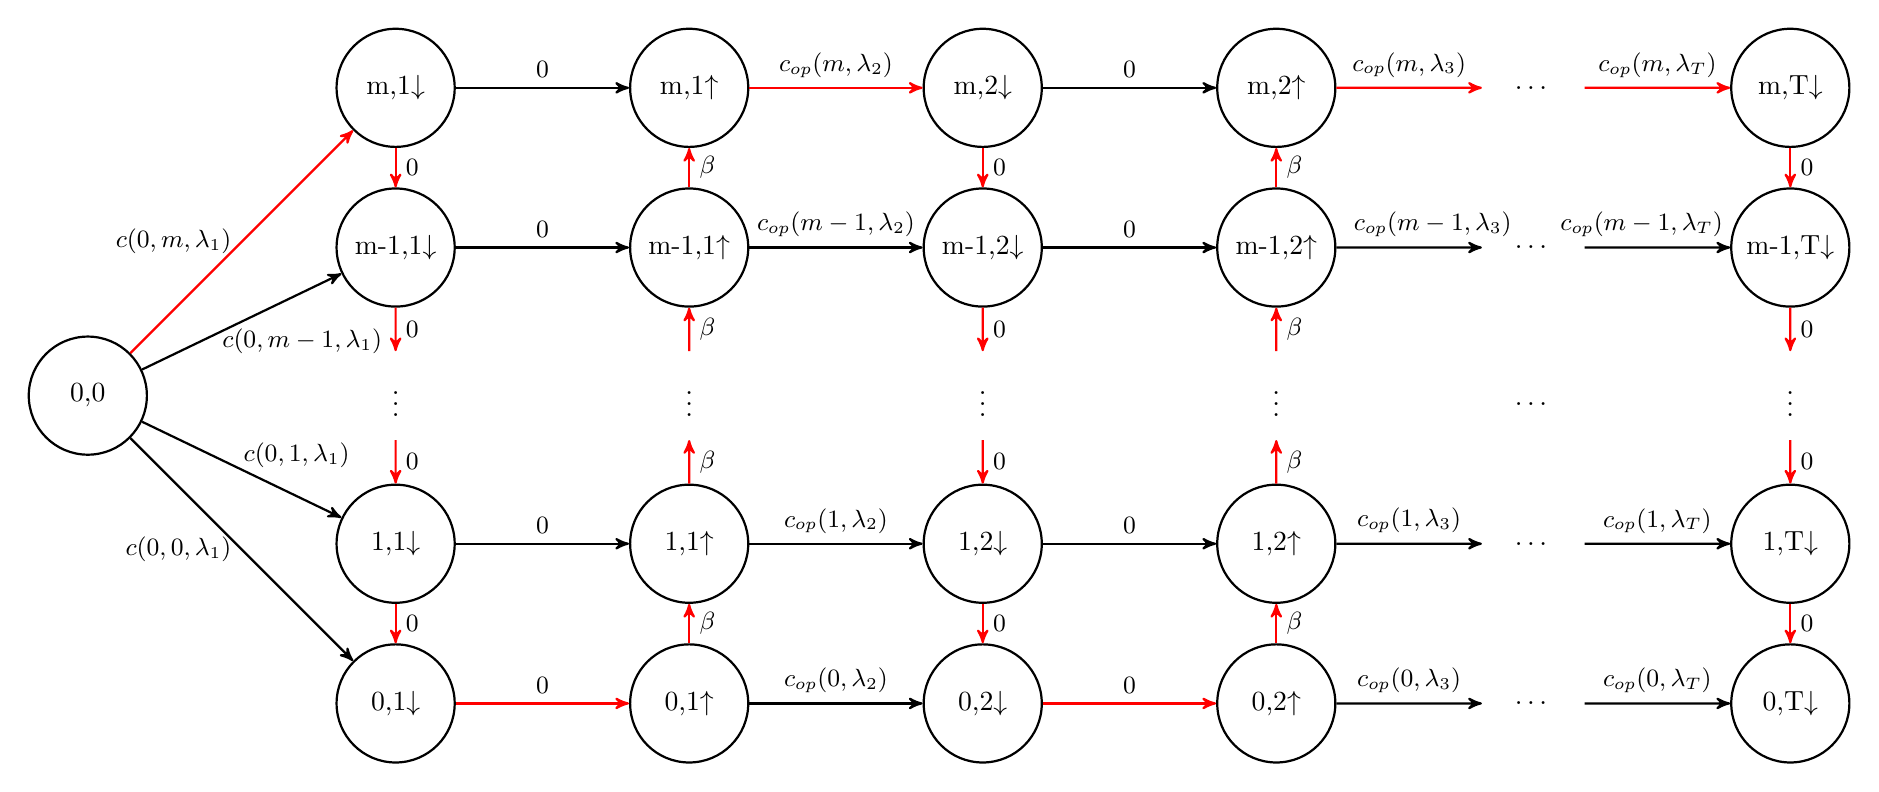
\begin{tikzpicture}[->,>=stealth',auto,node distance=2.2cm,thick,node/.style={minimum size=1.5cm,circle,draw}]
  \node[node] (1) {0,0};
  \node[node] (4) [below right=4cm of 1] {0,1$\downarrow$};
  \node[node] (3) [above =0.5cm of 4] {1,1$\downarrow$};
  \node[node] (2) [above right=4cm of 1] {m,1$\downarrow$};
  \node[node] (5) [below =0.5cm of 2] {m-1,1$\downarrow$};
  \node[node] (7) [right =of 3] {1,1$\uparrow$};
  \node[node] (6) [right =of 2] {m,1$\uparrow$};
  \node[node] (8) [right =of 4] {0,1$\uparrow$};
  \node[node] (9) [right =of 5] {m-1,1$\uparrow$};
  \node[node] (11) [right =of 7] {1,2$\downarrow$};
  \node[node] (10) [right =of 6] {m,2$\downarrow$};
  \node[node] (12) [right =of 8] {0,2$\downarrow$};
  \node[node] (13) [right =of 9] {m-1,2$\downarrow$};
  \node[node] (15) [right =of 11] {1,2$\uparrow$};
  \node[node] (14) [right =of 10] {m,2$\uparrow$};
  \node[node] (16) [right =of 12] {0,2$\uparrow$};
  \node[node] (17) [right =of 13] {m-1,2$\uparrow$};
  \node[node] (19) [right =5cm of 15] {1,T$\downarrow$};
  \node[node] (18) [right =5cm of 14] {m,T$\downarrow$};
  \node[node] (20) [right =5cm of 16] {0,T$\downarrow$};
  \node[node] (21) [right =5cm of 17] {m-1,T$\downarrow$};

  \node at ($(14)!.5!(18)$) {\ldots};
  \node (23) at ($(15)!.5!(19)$) {\ldots};
  \node at ($(16)!.5!(20)$) {\ldots};
  \node at ($(17)!.5!(21)$) {\ldots};
  \node [above =1.48cm of 23] {\ldots};

  \node at ($(2)!.5!(4)$) {\vdots};
  \node at ($(6)!.5!(8)$) {\vdots};
  \node at ($(10)!.5!(12)$) {\vdots};
  \node at ($(14)!.5!(16)$) {\vdots};
  \node at ($(18)!.5!(20)$) {\vdots};

  \path[every node/.style={font=\sffamily\small}]
    (1) edge[red] node[black,left] {$\costs(0,m,\lambda_1)$} (2)
	edge node[label={[xshift=0.9cm, yshift=-0.8cm]$\costs(0,m-1,\lambda_1)$}] {} (5)
	edge node[above right=-0.15cm] {$\costs(0,1,\lambda_1)$} (3)
	edge node[left] {$\costs(0,0,\lambda_1)$} (4)

    (2) edge node[above] {$0$} (6)
    (3) edge node[above] {$0$} (7)
    (4) edge[red] node[black,above] {$0$} (8)
    (5) edge node[above] {$0$} (9)

    (2) edge[red] node[black,right] {$0$} (5)
    (3) edge[red] node[black,right] {$0$} (4)

    (9) edge[red] node[black,right] {$\beta$} (6)
    (8) edge[red] node[black,right] {$\beta$} (7)

    (6) edge[red] node[black,above] {$\opcosts(m,\lambda_2)$} (10)
    (7) edge node[above] {$\opcosts(1,\lambda_2)$} (11)
    (8) edge node[above] {$\opcosts(0,\lambda_2)$} (12)
    (9) edge node[above] {$\opcosts(m-1,\lambda_2)$} (13)

    (10) edge node[above] {$0$} (14)
    (11) edge node[above] {$0$} (15)
    (12) edge[red] node[black,above] {$0$} (16)
    (13) edge node[above] {$0$} (17)

    (10) edge[red] node[black,right] {$0$} (13)
    (11) edge[red] node[black,right] {$0$} (12)

    (17) edge[red] node[black,right] {$\beta$} (14)
    (16) edge[red] node[black,right] {$\beta$} (15)

    (5) edge[red] node[black,right] {$0$} ($(5)!.35!(3)$)
    ($(5)!.65!(3)$) edge[red] node[black,right] {$0$} (3)

    ($(7)!.65!(9)$) edge[red] node[black,right] {$\beta$} (9)
    (7) edge[red] node[black,right] {$\beta$} ($(7)!.35!(9)$)
 
    (13) edge[red] node[black,right] {$0$} ($(13)!.35!(11)$)
    ($(13)!.65!(11)$) edge[red] node[black,right] {$0$} (11)

    ($(15)!.65!(17)$) edge[red] node[black,right] {$\beta$} (17)
    (15) edge[red] node[black,right] {$\beta$} ($(15)!.35!(17)$)


    (14) edge[red] node[label={[black,xshift=0cm, yshift=-0.26cm]$\opcosts(m,\lambda_3)$}] {} ($(14)!.4!(18)$)
    (15) edge node[label={[xshift=0cm, yshift=-0.26cm]$\opcosts(1,\lambda_3)$}] {} ($(15)!.4!(19)$)
    (16) edge node[label={[xshift=0cm, yshift=-0.26cm]$\opcosts(0,\lambda_3)$}] {} ($(16)!.4!(20)$)
    (17) edge node[label={[xshift=0.3cm, yshift=-0.26cm]$\opcosts(m-1,\lambda_3)$}] {} ($(17)!.4!(21)$)

    ($(14)!.6!(18)$) edge[red] node[black,above] {$\opcosts(m,\lambda_T)$} (18)
    ($(15)!.6!(19)$) edge node[above] {$\opcosts(1,\lambda_T)$} (19)
    ($(16)!.6!(20)$) edge node[above] {$\opcosts(0,\lambda_T)$} (20)
    ($(17)!.6!(21)$) edge node[label={[xshift=-0.2cm, yshift=-0.26cm]$\opcosts(m-1,\lambda_T)$}] {} (21)

    (18) edge[red] node[black,right] {$0$} (21)
    (19) edge[red] node[black,right] {$0$} (20)
    (21) edge[red] node[black,right] {$0$} ($(21)!.35!(19)$)
    ($(21)!.65!(19)$) edge[red] node[black,right] {$0$} (19);
\end{tikzpicture}
}
\caption{Graph for a pseudo-linear, optimal offline algorithm; the path of the topological sorting is highlighted in red.}
\label{fig_graph_pseudo_lin}
\end{figure}
For any possible amount of active servers $x$ and any time slot $t$, we add a node $v_{x,t\downarrow}$. Semantically, the cost of $v_{x,t\downarrow}$ will denote the minimum cost up to time slot $t$ when processing $\lambda_t$ with $x$ or more servers. Further, for any time slot $t\in[T-1]$ we add a node $v_{x,t\uparrow}$. The cost of $v_{x,t\uparrow}$ will denote the minimum cost of having $x$ active servers at the end of time slot $t$. Moreover, we add a start node $v_{0,0}$. Our end node will be $v_{0,T\downarrow}$.

The set of edges $E_s$ denotes the start initialisation step. An edge $(v_{x,t\uparrow},v_{x,t+1\downarrow})\in E_{\uparrow\downarrow}$ accounts for the operating costs that incur when processing the arrival rate $\lambda_{t+1}$ with $x$ active servers.

After any time step from $t-1$ to $t$ that incurs operating costs, we have a minimisation step in our graph. For this, we first move down the chain $v_{m,t\downarrow},v_{m-1,t\downarrow},\ldots,v_{0,t\downarrow}$ using edges from $E_\downarrow$ with cost $0$. Then we proceed to move to the right from $v_{0,t\downarrow}$ to $v_{0,t\uparrow}$. Lastly, we move up the chain $v_{0,t\uparrow},v_{1,t\uparrow},\ldots,v_{m,t\uparrow}$ using edges from $E_\uparrow$ with cost $\beta$. In order to have the possibility to keep the calculated costs of $v_{x,t\downarrow}$ during the upward movement, we add edges $(v_{x,t\downarrow},v_{x,t\uparrow})\in E_{\downarrow\uparrow}$ with cost $0$.

This minimisation step is the key to our runtime improvement. It facilitates the determination of the best predecessor of a state $v_{x,t\downarrow}$ because we already know that the minimum cost of having $x$ servers at the end of time slot $t-1$ is stored in $v_{x,t-1\uparrow}$. Thus, the cheapest possibility to process the next arrival rate $\lambda_t$ using $x$ servers can simply be calculated by adding $\opcosts(x,\lambda_t)$ to the cost of $v_{x,t-1\uparrow}$. Consequently, the cost of $v_{x,t\downarrow}$ is given by the minimum of $v_{x,t-1\uparrow}+\opcosts(x,\lambda_t)$ and $v_{x+1,\downarrow}$.

As one can see in Figure~\ref{fig_graph_pseudo_lin}, we stretched our graph but at the same time also greatly reduced the amount of edges compared to our initial approach in section~\ref{sec_opt_offline_pseudo_poly}. By following the coloured path of the topological sorting, we can work our way through the graph to calculate the shortest paths, ultimately reaching the destination $v_{0,T\downarrow}$. The cost of our destination $v_{0,T\downarrow}$ will denote the minimum cost up to time slot $T$ when processing $\lambda_T$ with 0 or more servers. Hence, it will contain our desired end result --- the minimum cost of all possible schedules.

Our next task shall be the verification of our new construction. For this, we first examine the possible paths from $v_{0,0}$ to $v_{0,T\downarrow}$ in our graph.
In contrast to our approach in section~\ref{sec_opt_offline_pseudo_poly}, our new graph contains paths that do not directly correspond to a schedule $\mx$. For example, consider the following path:
\begin{equation*}
	P\coloneqq(v_{0,0},v_{1,1\downarrow},v_{0,1\downarrow},v_{0,1\uparrow},v_{1,1\uparrow},v_{2,1\uparrow},v_{2,2\downarrow},\ldots,v_{0,T\downarrow})
\end{equation*}
A schedule corresponding to $P$ would use one active server in its first time slot, then power down this server, and subsequently turn on two servers to process the next arrival rate. This seems somewhat unreasonable. We could just keep the initial server on to save switching costs (note the correspondence to Proposition~\ref{prop_reasonable_switching}). In fact, this behaviour cannot even be represented using our schedule notation $\mx$ and optimisation condition~\eqref{eq_even_distribution_schedule_costs}. We can, however, modify $P$ to represent a more reasonable sequence, that is we set
\begin{equation*}
	P'\coloneqq(v_{0,0},v_{1,1\downarrow},v_{1,1\uparrow},v_{2,1\uparrow},v_{2,2\downarrow},\ldots,v_{0,T\downarrow})
\end{equation*}
This revised path now pleasantly translates to a schedule $\mx$, in this case $\mx=(1,2,\ldots)$. We now want to give a more formal definition of our observation.
\begin{defn}[reasonable paths]\label{defn_reasn_paths}
Let $P$ be a path from $v_{0,0}$ to $v_{0,T\downarrow}$. For any time slot $t\in[T]$, let $E_\downarrow^t$ be the set of edges $(v_{x,t\downarrow},v_{x-1,t\downarrow})\in E_\downarrow$ used by $P$ at time $t$. Similarly, let $E_\uparrow^t$ be the set of edges $(v_{x,t\uparrow},v_{x+1,t\uparrow})\in E_\uparrow$ used by $P$ at time $t\in[T-1]$.
The path $P$ is called \textit{reasonable} if for any time slot $t\in[T-1]$, the path does not shut down and power on servers simultaneously at $t$. More formally, $P$ must satisfy the formula
\begin{equation}
	\forall t\in[T-1]\left(E_\downarrow^t=\emptyset \lor E_\uparrow^t=\emptyset\right)\label{eq_reasn_path}
\end{equation}
\end{defn}
Using this definition, we can now verify that our reasonable paths indeed deserve to be called \textit{reasonable}.
\begin{prop}\label{prop_path_to_reasn_path}
Any given path $P$ from $v_{0,0}$ to $v_{0,T\downarrow}$ can be transformed to a reasonable path $P'$ with $\costs(P')\le\costs(P)$.
\end{prop}
\begin{proof}
Let $P$ be a path from $v_{0,0}$ to $v_{0,T\downarrow}$. We give a procedure that repeatedly modifies $P$ such that it satisfies~\eqref{eq_reasn_path} and reduces or retains its costs. 

Let $t\in[T-1]$ be the first time slot falsifying~\eqref{eq_reasn_path}. If there does not exist such a time slot, we are done. Otherwise, let $E_\downarrow^t$ and $E_\uparrow^t$ be its sets of edges as defined in Definition~\ref{defn_reasn_paths}. Since $P$ falsifies~\eqref{eq_reasn_path} at time $t$, both $E_\downarrow^t$ as well as $E_\uparrow^t$ must be non-empty. Thus, we can obtain the ``maximum'' nodes involved in these sets.
\begin{align*}
	x_s\coloneqq&\max\bigl\{x\in[m]\mid (v_{x,t\downarrow},v_{x-1,t\downarrow})\in E_\downarrow^t\bigr\}\\
	x_e\coloneqq&\max\bigl\{x\in[m]\mid (v_{x-1,t\uparrow},v_{x,t\uparrow})\in E_\uparrow^t\bigr\}
\end{align*}
Next, consider the subpath $S=(v_{x_s,t\downarrow},\ldots,v_{x_e,t\uparrow})$ of $P$. Note that the subpath in particular uses all edges from $E_\downarrow^t$ and $E_\uparrow^t$.
Naturally, a most cost-efficient path $S'$ from node $v_{x_s,t\downarrow}$ to $v_{x_e,t\uparrow}$ minimises the number of edges $(v_{x,t\uparrow},v_{x+1,t\uparrow})$ since each of these edges incurs cost $\beta\ge 0$. For this, we observe that we must not shut down servers if $x_s\le x_e$, and that we must not power on servers if $x_s\ge x_e$; thus, we consider three cases for $S'$:
\begin{equation*}
	S'\coloneqq
	\begin{cases}
		(v_{x_s,t\downarrow},v_{x_s,t\uparrow},v_{x_s+1,t\uparrow},\ldots,v_{x_e,t\uparrow}), & \text{if $x_s< x_e$}\\
		(v_{x_s,t\downarrow},v_{x_s-1,t\downarrow},\ldots,v_{x_e,t\downarrow},v_{x_e,t\uparrow}), & \text{if $x_s>x_e$}\\
		(v_{x_s,t\downarrow},v_{x_e,t\uparrow}), & \text{if $x_s=x_e$}
	\end{cases}
\end{equation*}
In each case, $S'$ uses edges from at most one of the sets $E_\downarrow^t$ and $E_\uparrow^t$. Thus, by replacing the subpath $S$ of $P$ with $S'$, we obtain a new schedule $P'$ that satisfies~\eqref{eq_reasn_path} up to and including time slot $t$. Moreover, the paths $P$ and $P'$ coincide in their costs before visiting $v_{x_s,t\downarrow}$ and after visiting $v_{x_e,t\uparrow}$; however, they differ in that there are less switching costs $\beta$ at time $t$ using $P'$. As we assume $\beta\ge0$, we conclude $\costs(P')\le \costs(P)$.

Hence, by repeating described process on $P'$, we obtain a terminating procedure that returns a path satisfying the conditions.
\end{proof}
\begin{lem}\label{lem_sched_path_pseudo_lin}
Let $\bm{\mx}$ be the set of all schedules $\mx$ for $\inp$, and let $\bm{\mathcal{P}}$ the set of all reasonable paths. There exists a bijective map $\Phi:\bm{\mathcal{P}}\rightarrow\bm{\mx}$ satisfying $\costs(P)=\costs\bigl(\Phi(P)\bigr)$.
\end{lem}
\begin{proof}
TODO

Which shows that $\Phi$ is a cost-preserving maps, and the claim follows.
\end{proof}
\begin{thm}\label{thm_opt_sched_reasn_path}
There is a cost-preserving bijection between optimal schedules $\mx$ for $\inp$ and shortest, reasonable paths.
\end{thm} 
\begin{proof}
By Lemma~\ref{lem_sched_path_pseudo_lin}, we have a bijection $\Phi$ between reasonable paths $P$ and schedules $\mx$ obeying $\costs(P)=\costs\bigl(\Phi(P)\bigr)$. Thus, we have 
\begin{equation*}
	\costs(P)\text{ minimal}\iff \costs\bigl(\Phi(P)\big)\text{ minimal}
\end{equation*}
and the claim follows.
\end{proof}
\begin{cor}
Any shortest path $P$ from $v_{0,0}$ to $v_{0,T\downarrow}$ can be transformed to an optimal schedule $\mx$ for $\inp$ with $\costs(\mx)=\costs(P)$.
\end{cor}
\begin{proof}
Let $P$ be a shortest path from $v_{0,0}$ to $v_{0,T\downarrow}$. By Proposition~\ref{prop_path_to_reasn_path}, the path $P$ can be transformed to a reasonable path $P'$ with $\costs(P')=\costs(P)$.
In turn, $P'$ corresponds to an optimal schedule $\mx$ with $\costs(\mx)=\costs(P')$ by Theorem~\ref{thm_opt_sched_reasn_path}. Thus, we have $c(\mx)=c(P)$ and, the claim follows.
\end{proof}

\section{Approximative offline scheduling}
\subsection{A polynomial $4$-approximation algorithm}
%We consider a modification of the problem discussed in chapter. Assuming that f is convex and monotonically increasing, we can modify our algorithm to obtain a polynomial time $4$-approximation algorithm.

%We modify our graph from section~\ref{sec_opt_offline_pseudo_poly} to the reduce the number of nodes. For this, we stop adding m nodes for each timestep, but use nodes that approximate the number of active servers instead. First, let $b\coloneqq\lceil\log_2(m)\rceil$. We add nodes $(t,0)$ and $(t,2^i),\forall t\in[T-1],0\le i\le b$. All edges and weights are added analogous to chapter~\ref{sec_opt_offline_pseudo_poly}.
%\begin{figure}[H]
%\begin{tikzpicture}[->,>=stealth',auto,node distance=3cm,thick,node/.style={minimum size=1.2cm,circle,draw}]

  %\node[node] (1) {0,0};
  %\node[node] (4) [below right =of 1] {1,0};
  %\node[node] (3) [above =0.5cm of 4] {1,$2^0$};
  %\node[node] (2) [above right=of 1] {1,$2^b$};
  %\node[node] (6) [right =of 3] {2,$2^0$};
  %\node[node] (5) [right =of 2] {2,$2^b$};
  %\node[node] (7) [right =of 4] {2,0};
  %\node[node] (9) [right =of 6] {T-1,$2^0$};
  %\node[node] (8) [right =of 5] {T-1,$2^b$};
  %\node[node] (10) [right =of 7] {T-1,0};
  %\node[node] (11) [above right =of 10] {T,0};

  %\node at ($(5)!.4!(8)$) {\ldots};
  %\node at ($(6)!.4!(9)$) {\ldots};
  %\node at ($(7)!.4!(10)$) {\ldots};

  %\node at ($(2)!.5!(3)$) {\vdots};
  %\node at ($(2)!.5!(6)$) {\vdots};
  %\node at ($(5)!.5!(6)$) {\vdots};
  %\node at ($(8)!.5!(9)$) {\vdots};

  %\path[every node/.style={font=\sffamily\small}]
    %(1) edge node[left] {$d(0,2^b,\lambda_1)$} (2)
	%edge node[above right=-0.1cm] {$d(0,2^0,\lambda_1)$} (3)
	%edge node[left] {$d(0,0,\lambda_1)$} (4)
    %(2) edge node[above] {$d(2^b,2^b,\lambda_2)$} (5)
    %(3) edge (6)
	%edge (7)
    %(4) edge (6)
	%edge node[below] {$d(0,0,\lambda_2)$} (7)
    %(8) edge node[right] {$0$} (11)
    %(9) edge node[above] {$0$} (11)
    %(10) edge node[above] {$0$} (11);

   %\path [->,draw,thick] (1) to ($(1)!.2!(8)$);
   %\path [->,draw,thick] (2) to ($(2)!.4!(6)$);
   %\path [->,draw,thick] (4) to ($(4)!.4!(5)$);
   %\path [->,draw,thick] (3) to ($(3)!.4!(5)$);

   %\path [->,draw,thick] ($(3)!.6!(5)$) to (5);
   %\path [->,draw,thick] ($(2)!.6!(6)$) to (6);
   %\path [->,draw,thick] ($(2)!.6!(7)$) to (7);

   %\path [->,draw,thick] ($(6)!.6!(8)$) to (8);
   %\path [->,draw,thick] ($(5)!.6!(8)$) to (8);

   %\path [->,draw,thick] ($(5)!.6!(9)$) to (9);
   %\path [->,draw,thick] ($(6)!.6!(9)$) to (9);
   %\path [->,draw,thick] ($(7)!.6!(9)$) to (9);

   %\path [->,draw,thick] ($(5)!.6!(10)$) to (10);
   %\path [->,draw,thick] ($(6)!.6!(10)$) to (10);
   %\path [->,draw,thick] ($(7)!.6!(10)$) to (10);

   %\path[every node/.style={font=\sffamily\small}] [->,draw,thick] ($(2)!.8!(11)$) -- node[above] {0} ++ (11);

%\end{tikzpicture}
%\caption{Graph for a $4$-approximation algorithm}
%\end{figure}

%\begin{defn}
%Let $\mx=(x_0,\ldots,x_T)$ be a schedule and $t>0$.\\
%We say that $\mx$ changes its \textbf{state} at time t if
%\begin{equation*}
	%x_t\neq x_{t-1}
%\end{equation*}
%and that $\mx$ changes its \textbf{2-state} at time t if
%\begin{equation*}
	%x_t=0\text{\quad or\quad}x_t\notin\bigl(2^{\lfloor \log_2(x_{t-1})\rfloor},2^{\lceil \log_2(x_{t-1})\rceil}\bigr)
%\end{equation*}
%\end{defn}
%\begin{prop}
%$ $
%\begin{enumerate}
	%\item\label{prop:2opt} Any given optimal schedule $\mx$ can be transformed to a $4$-optimal schedule $\mx'$ which corresponds to a path $P$ from $(0,0)$ to $(T,0)$ with $costs(\mx')=costs(P)$.
	%\item Any shortest path $P$ from $(0,0)$ to $(T,0)$ corresponds to a $4$-optimal schedule $\mx$ with $costs(P)=costs(\mx)$.
%\end{enumerate}
%\end{prop}
%\begin{proof}
%$ $
%\begin{enumerate}
	%\item Assume we have an optimal schedule identified by $\mx=(x_0,\ldots,x_T)$. For $0\le t<T$ we inductively set:
%\begin{equation}
	%x'_0\coloneqq 0,\qquad
	%x'_{t+1}\coloneqq 
	%\begin{cases}
		%\min\bigl\{2^{\lfloor \log_2(2x_{t+1})\rfloor},2^b\bigr\}, & \text{if $0<x_t\le x_{t+1}$}\\
		%2^{\lceil \log_2(2x_{t+1})\rceil}, & \text{if $0<x_{t+1}<x_t$ and $x'_{t}\ge4x_{t+1}$}\\
		%x'_t, & \text{if $0<x_{t+1}<x_t$ and $x'_{t}<4x_{t+1}$}\\
		%\		   0, & \text{otherwise}
	%\end{cases} \label{def:chi_prime}
%\end{equation}
%Then let $\mx'\coloneqq(x'_0,\ldots,x'_T)$ be the modified sequence of active servers. Notice that \makebox{$x_t\le x'_t\le 4x_t$} holds as $x'_t$ is at most the smallest power of two larger than $2x_t$ which implies that $\mx'$ is feasible.\\
%We can now construct a feasible path in our graph from $\mathcal{X'}$ as follows:
%\begin{align*}
	%\text{First set}&&e_t&\coloneqq\Bigl(\bigl(t,\mx'(t)\bigr),\bigl(t+1,\mx'(t+1)\bigr)\Bigr),&\forall t\in\fromto{0}{T-1}\\
	%\text{then set}&&P&\coloneqq(e_0,\ldots,e_{T-1})
%\end{align*}
%By the definition of the edges' weights it follows that $costs(\mx')=costs(P)$.\\
%Next, let $(t_0=0,t_1,\ldots,t_n=0)$ be the sequence of times where the optimal schedule $\mx$ changes its 2-state. Notice that the modified schedule $\mx'$ changes its state only at times $t_i$ and that $2x_{t_i}\le x'_{t_i}$ holds (TODO: only if not discrete but continous time steps). This can be seen exemplarily in figure~\ref{fig:adaption-schedule} by obvserving that $\mx'$ changes its state only if $\mx$ crosses or touches a bordering power of two.
%\begin{figure}[H]
%\centering
%\scalebox{0.7}{
%\subfloat{
%\begin{tikzpicture}
	%\begin{axis}[%
	    %,xlabel=$t$
	    %,axis x line = bottom,axis y line = left
	    %,ytick={1,2,4,8,16}
	    %,ymax=17 % or enlarge y limits=upper
	    %,xmax=9.9
	    %,legend pos=outer north east
	    %]
	%\addplot+[const plot, no marks, thick, color=blue] coordinates {(0,0) (1,5) (2,3) (3,7) (4,8) (5,5) (6,4) (7,3) (8,2) (9,0) (9.5,0)};
	%\addplot+[const plot, no marks, thick, color=red] coordinates {(0,0) (1,10) (2,6) (3,14) (4,16) (5,10) (6,8) (7,6) (8,4) (9,0) (9.5,0)};
	%\addplot+[const plot, no marks, thick, dotted, color=black] coordinates {(1,0) (1,8)};
	%\addplot+[const plot, no marks, thick, dotted, color=black] coordinates {(4,0) (4,16)};
	%\addplot+[const plot, no marks, thick, dotted, color=black] coordinates {(6,0) (6,8)};
	%\addplot+[const plot, no marks, thick, dotted, color=black] coordinates {(8,0) (8,4)};
	%\addplot+[const plot, no marks, thick, dashed, color=black] coordinates {(0,1) (9.5,1)};
	%\addplot+[const plot, no marks, thick, dashed, color=black] coordinates {(0,2) (9.5,2)};
	%\addplot+[const plot, no marks, thick, dashed, color=black] coordinates {(0,4) (9.5,4)};
	%\addplot+[const plot, no marks, thick, dashed, color=black] coordinates {(0,8) (9.5,8)};
	%\addplot+[const plot, no marks, thick, dashed, color=black] coordinates {(0,16) (9.5,16)};
	%\addlegendentry{$x_t$}
	%\addlegendentry{$2x_t$}
	%\end{axis}
%\end{tikzpicture}}}
%\qquad
%\scalebox{0.7}{
%\subfloat{
%\begin{tikzpicture}
	%\begin{axis}[%
	    %,xlabel=$t$
	    %,axis x line = bottom,axis y line = left
	    %,ytick={1,2,4,8,16}
	    %,ymax=17 % or enlarge y limits=upper
	    %,xmax=9.9
	    %,legend pos=outer north east
	    %]
	%\addplot+[const plot, no marks, thick, color=green] coordinates {(0,0) (1,8) (2,8) (3,8) (4,16) (5,16) (6,8) (7,8) (8,4) (9,0) (9.5,0)};
	%\addplot+[const plot, no marks, thick, dotted, color=black] coordinates {(1,0) (1,8)};
	%\addplot+[const plot, no marks, thick, dotted, color=black] coordinates {(4,0) (4,16)};
	%\addplot+[const plot, no marks, thick, dotted, color=black] coordinates {(6,0) (6,8)};
	%\addplot+[const plot, no marks, thick, dotted, color=black] coordinates {(8,0) (8,4)};
	%\addplot+[const plot, no marks, thick, dashed, color=black] coordinates {(0,1) (9.5,1)};
	%\addplot+[const plot, no marks, thick, dashed, color=black] coordinates {(0,2) (9.5,2)};
	%\addplot+[const plot, no marks, thick, dashed, color=black] coordinates {(0,4) (9.5,4)};
	%\addplot+[const plot, no marks, thick, dashed, color=black] coordinates {(0,8) (9.5,8)};
	%\addplot+[const plot, no marks, thick, dashed, color=black] coordinates {(0,16) (9.5,16)};
	%\addlegendentry{$x'_t$}
	%\end{axis}
%\end{tikzpicture}}}
 	%\caption{Adaption of an optimal schedule}
	%\label{fig:adaption-schedule}
%\end{figure}
	%For this reason, we now only have to consider the fraction of costs of $\mx'$ and $\mx$ between time steps $t_{i-1}$ and $t_i$
	%\begin{equation}
		%\frac{costs(\mx',t_{i-1},t_i)}{costs(\mx,t_{i-1},t_i)}\label{eq:frac_chi_prime}
	%\end{equation}
	%For $x_{t_i}=0$ it follows from \eqref{eq:costs_chi_t_t_prime} that $costs(\mx',t_{i-1},t_i)=costs(\mx,t_{i-1},t_i)=0$. Hence, we can restrict ourselves to $0<t_i<T$ with $x_{t_i}\neq 0$.
	%The costs incurred by $\mx'$ are given by
	%\begin{align}
		%&&costs(\mx',t_{i-1},t_i)&=\beta\max\{0,x'_{t_i}-x'_{t_{i-1}}\}+x'_{t_i}f(\lambda_{t_i}/x'_{t_i})&\text{by \eqref{eq:costs_chi_t_t_prime}}\nonumber\\
		%&&&\le\beta\max\{0,x'_{t_i}-x'_{t_{i-1}}\}+4x_{t_i}f(\lambda_{t_i}/x'_{t_i})&\text{by \eqref{def:chi_prime}}\nonumber\\
		%&&&\le\beta\max\{0,x'_{t_i}-x'_{t_{i-1}}\}+4x_{t_i}f(\lambda_{t_i}/x_{t_i})&\text{f monotonically increasing}\nonumber\\
		%\implies&&costs(\mx',t_{i-1},t_i)&\le\beta\max\{0,x'_{t_i}-x'_{t_{i-1}}\}+4x_{t_i}f(\lambda_{t_i}/x_{t_i})\label{eq:est_chi_prime}
	%\end{align}
	%and the costs of $\mx$ by
	%\begin{equation}
		%costs(\mx,t_{i-1},t_i)=\beta\max\{0,x_{t_i}-x_{t_{i-1}}\}+x_{t_i}f(\lambda_{t_i}/x_{t_i})\label{eq:optcosts}
	%\end{equation}
	%W.l.o.g.\ we may assume $x_{t_i}f(\lambda_{t_i}/x_{t_i})>0$, otherwise the claim follows trivially. (TODO: is it really trivial?)
	%\begin{enumerate}[(i)]
		%\item\label{pr:4appr_1} \underline{$x_{t_i}\le x_{t_{i-1}}$:}
			%From~\eqref{def:chi_prime} it follows that $x'_{t_i}\le x'_{t_{i-1}}$. Thus, we can simplify~\eqref{eq:frac_chi_prime}:
		%\begin{align*}
			%\frac{costs(\mx',t_{i-1},t_i)}{costs(\mx,t_{i-1},t_i)}&\le\frac{\beta\max\{0,x'_{t_i}-x'_{t_{i-1}}\}+4x_{t_i}f(\lambda_{t_i}/x_{t_i})}{\beta\max\{0,x_{t_i}-x_{t_{i-1}}\}+x_{t_i}f(\lambda_{t_i}/x_{t_i})}&\text{by \eqref{eq:est_chi_prime},\eqref{eq:optcosts}}\\
			%&=\frac{4x_{t_i}f(\lambda_{t_i}/x_{t_i})}{x_{t_i}f(\lambda_{t_i}/x_{t_i})}&\text{($x_{t_i}\le x_{t_{i-1}}$ and $x'_{t_i}\le x'_{t_{i-1}}$)}\\
			%&=4
		%\end{align*}
		%\item\label{pr:4appr_2} \underline{$x_{t_i}>x_{t_{i-1}}$:}
		%From (\ref{def:chi_prime}) it follows that $x'_{t_i}\ge x'_{t_{i-1}}$. Thus, we can simplify~(\ref{eq:frac_chi_prime}):
		%\begin{align*}
			%\frac{costs(\mx',t_{i-1},t_i)}{costs(\mx,t_{i-1},t_i)}&\le\frac{\beta\max\{0,x'_{t_i}-x'_{t_{i-1}}\}+4x_{t_i}f(\lambda_{t_i}/x_{t_i})}{\beta\max\{0,x_{t_i}-x_{t_{i-1}}\}+x_{t_i}f(\lambda_{t_i}/x_{t_i})}&\text{by \eqref{eq:est_chi_prime},\eqref{eq:optcosts}}\\
			%&=\frac{\beta(x'_{t_i}-x'_{t_{i-1}})+4x_{t_i}f(\lambda_{t_i}/x_{t_i})}{\beta(x_{t_i}-x_{t_{i-1}})+x_{t_i}f(\lambda_{t_i}/x_{t_i})}&\text{($x_{t_i}>x_{t_{i-1}}$ and $x'_{t_i}\ge x'_{t_{i-1}}$)}\\
			%&=\frac{\beta(\min\bigl\{2^{\lfloor \log_2(2x_{t_i})\rfloor},2^b\bigr\}-x'_{t_{i-1}})+4x_{t_i}f(\lambda_{t_i}/x_{t_i})}{\beta(x_{t_i}-x_{t_{i-1}})+x_{t_i}f(\lambda_{t_i}/x_{t_i})}&\text{by \eqref{def:chi_prime}}\\
			%&\le\frac{\beta(2^{\lfloor \log_2(2x_{t_i})\rfloor}-x'_{t_{i-1}})+4x_{t_i}f(\lambda_{t_i}/x_{t_i})}{\beta(x_{t_i}-x_{t_{i-1}})+x_{t_i}f(\lambda_{t_i}/x_{t_i})}\\
			%&\le\frac{\beta(2x_{t_i}-x'_{t_{i-1}})+4x_{t_i}f(\lambda_{t_i}/x_{t_i})}{\beta(x_{t_i}-x_{t_{i-1}})+x_{t_i}f(\lambda_{t_i}/x_{t_i})}\\
			%&\le\frac{\beta(2x_{t_i}-2x_{t_{i-1}})+4x_{t_i}f(\lambda_{t_i}/x_{t_i})}{\beta(x_{t_i}-x_{t_{i-1}})+x_{t_i}f(\lambda_{t_i}/x_{t_i})}&\text{by ($2x_{t_{i-1}}\le x'_{t_{i-1}}$)}\\
			%&\le4\ \frac{\frac{1}{2}\beta(x_{t_i}-x_{t_{i-1}})+x_{t_i}f(\lambda_{t_i}/x_{t_i})}{\ \ \beta(x_{t_i}-x_{t_{i-1}})+x_{t_i}f(\lambda_{t_i}/x_{t_i})}\\
			%&\le4
		%\end{align*}
	%\end{enumerate}
	%From~(\hyperref[pr:4appr_1]{i}) and~(\hyperref[pr:4appr_2]{ii}) it follows:
	%\begin{equation*}
		%costs(\mx')\le4costs(\mx)
	%\end{equation*}
	%\item From~\ref{prop:2opt} we obtain that we can construct a $4$-optimal path $P'$ from any optimal schedule. Now, let $P$ be a shortest path. We have $costs(P)\le costs(P')<\infty$, and since every path $P$ with $costs(P)<\infty$ corresponds to a feasible schedule $\mx$ with $costs(P)=costs(\mx)$, $\mx$ must also be at least $4$-optimal.
%\end{enumerate}
%\end{proof}

%\newpage
%\bibliographystyle{plain}
%\bibliography{sources.bib}
\newpage

\section*{Appendix}
Below, we give an overview of just given definitions and conventions commonly referred to in our paper:
%\scriptsize
%\begin{multicols}{2}
\begin{itemize}
\item Input:
\begin{itemize}
	\item $m\in\mathbb{N}$\ldots number of homogeneous servers
	\item $T\in\mathbb{N}$\ldots number of time slots
	\item $\lambda_1,\ldots,\lambda_{T}\in[0,m]$\ldots arrival rates
	\item $\Lambda\coloneqq(\lambda_1,\ldots,\lambda_T)$\ldots sequence of arrival rates
	\item $\beta\in\mathbb{R}_{\ge 0}$\ldots switching costs of a server
	\item $f:[0,1]\rightarrow\mathbb{R}$\ldots convex operating costs function of a server
	\item $\inp\coloneqq(m,T,\Lambda,\beta,f)$\ldots input of a problem instance
\end{itemize}

\item Problem statement:
\begin{itemize}
	\item $s_{i,t}\in\{0,1\}$\ldots state of server $i$ at time $t$, i.e.\ sleeping (0) or active(1)
	\item $S_i\coloneqq(s_{i,1},\ldots,s_{i,T})$\ldots sequence of states for server $i$
	\item $\lambda_{i,t}\in[0,1]$\ldots assigned load for server $i$ at time $t$
	\item $L_i\coloneqq(\lambda_{i,1},\ldots,\lambda_{i,T})$\ldots sequence of assigned loads for server $i$
	\item $\mathcal{S}\coloneqq(S_1,\ldots,S_m)$\ldots sequence of all state changes
	\item $\mathcal{L}\coloneqq(L_1,\ldots,L_m)$\ldots sequence of all assigned loads
	\item $\Sigma\coloneqq(\mathcal{S},\mathcal{L})$\ldots schedule for a problem instance $\inp$
\end{itemize}

\item Miscellaneous:
\begin{itemize}
	\item $x_t\in\fromto{0}{m}$\ldots number of active servers at time t
	\item $\mx\coloneqq(x_1,\ldots,x_T)$\ldots sequence of number of active servers
\end{itemize}

\item Conventions:
\begin{itemize}
	\item $\lambda_{t}=0$ for all $t\notin[T]$, i.e.\ there is no load before and after the scheduling process
	\item $s_{i,t}=0$ for all $t\notin[T]$, i.e.\ all servers are powered down before and after the scheduling process
\end{itemize}
\end{itemize}
%\end{multicols}
\normalsize

\end{document}
